\subsection{复形的运算}

在集合 A × A 上，这两个运算

\[
\begin{array}{l} (a, b) + (a ^ {\prime}, b ^ {\prime}) = (a + a ^ {\prime}, b + b ^ {\prime}) \\ (a, b) (a ^ {\prime}, b ^ {\prime}) = (a a ^ {\prime}, a b ^ {\prime} + b a ^ {\prime}) \end{array}
\]

定义一个环结构，记为 A(ε)，其单位元为 1 = (1, 0)；嵌入映射 a ↦ (a, 0) = a1 使得 A 可被等同于 A(ε) 的一个子环；模 A(ε) 是自由的，其基为 \{ 1, ε \} 其中 ε = (0, 1)；我们有 ε² = 0，且 ε 在 A(ε) 中是中心的。

当A是交换的时， \(\mathrm{A}(\varepsilon)\) 是 A 上的双数代数（III，第 15 页）。赋予 \(\mathrm{A}(\varepsilon)\) 环分次结构（II，第164页），其中 \(\mathrm{A}(\varepsilon)_{0} = \mathrm{A}.1\) , \(\mathrm{A}(\varepsilon)_{-1} = \mathrm{A}. \varepsilon\) ，且 \(\mathrm{A}(\varepsilon)_{n} = 0\) （当 \(n \neq 0, -1\) ）。显然，在一个集合 C 上给出 A-复形结构，等同于在 C 上给出一个 \(\mathrm{A}(\varepsilon)\) 分次模结构，其中微分 d 对应于位似 \(\varepsilon_{C}\) ；同样地，复形的态射对应于 \(\mathrm{A}(\varepsilon)\) 分次模的次数为 0 的分次同态。因此， \(\mathrm{A}(\varepsilon)\) 分次模与 A-复形的结构种类是等价的（E, IV, 第 9-10 页）。我们将利用这一事实，将分次模理论中的通常概念移植到复形理论中。

对于分次子 A(ε)-模的概念，对应的是子复形的概念：因此，复形 (C, d) 的子复形是 C 的一个分次子模 C'，使得对每个 \(n \in Z\) , \(d_{n}(C_{n}') \subset C_{n-1}'\) ；若用 \(d'\) 表示由 d 诱导的从 C' 到 C' 的分次 A-同态，则 (C', d') 是一个复形结构，称为由 (C, d) 诱导的结构。除非另有明确说明，每个子复形都配备诱导结构。

我们将其留给读者，按照下面的词典，类似地详细阐述复形的商复形、复形的正合列、复形态射的核、余核和像的概念：

分次商 A(ε)-模

= 商复形，

次数为 0 的分次 A(ε)-同态的核、余核、像 \} 复形态射的核、余核、像，

分次A(ε)-模的正合列以及次数为0的分次同态 \} = 复形的正合列。

例如，第 1 号中的典范正合列给出复形的正合列，称为典范的。

\begin{enumerate}
\def\labelenumi{(\Roman{enumi})}
\tightlist
\item
\end{enumerate}

\[
0 \longrightarrow \mathrm{Z} (\mathrm{C}) \longrightarrow \mathrm{C} \stackrel {\delta} {\longrightarrow} \mathrm{B} (\mathrm{C}) (- 1) \longrightarrow 0,\tag{II}
\]

\[
0 \longrightarrow \mathrm{B} (\mathrm{C}) \longrightarrow \mathrm{Z} (\mathrm{C}) \longrightarrow \mathrm{H} (\mathrm{C}) \longrightarrow 0,\tag{III}
\]

\[
0 \longrightarrow \mathrm{B} (\mathrm{C}) \longrightarrow \mathrm{C} \longrightarrow \mathrm{C} / \mathrm{B} (\mathrm{C}) \longrightarrow 0,\tag{IV}
\]

\[
0 \longrightarrow \mathrm{H} (\dot {\mathrm{C}}) \longrightarrow \mathrm{C} / \mathrm{B} (\mathrm{C}) \stackrel {\delta} {\longrightarrow} \mathrm{B} (\mathrm{C}) (- 1) \stackrel {\cdot} {\longrightarrow} 0,\tag{V}
\]

\[
0 \longrightarrow \mathrm{H} (\mathrm{C}) \longrightarrow \mathrm{C} / \mathrm{B} (\mathrm{C}) \longrightarrow \mathrm{Z} (\mathrm{C}) (- 1) \longrightarrow \mathrm{H} (\mathrm{C}) (- 1) \longrightarrow 0.
\]

类似地，可以定义复形的直和、复形的归纳系以及复形的归纳系的归纳极限等概念。

设 \((\mathbf{C}_{i}, d_{i})\) 为一族复形。称此族的积，并记作 \(\prod_{i \in I} (\mathbf{C}_{i}, d_{i})\)，是按如下方式得到的复形 \((\mathbf{C}, d)\)：

\begin{enumerate}
\def\labelenumi{\alph{enumi})}
\item
  对于每个 \(n \in Z\) , \(C_{n}\) 是直积 A-模 \(\prod_{i \in I} (\mathbf{C}_{i})_{n}\)，即给定复形的齐次分量 \((\mathbf{C}_{i})_{n}\) 的直积
\item
  对于每个 \(n \in Z\) , \(d_{n} : C_{n} \to C_{n-1}\) 是A-同态，其分量为 \((d_{i})_{n}\) .
\end{enumerate}

当 I 有限时， \(\prod_{i\in I}(\mathbf{C}_{i},d_{i})\) 等于 \(\bigoplus_{i\in I}(\mathbf{C}_{i},d_{i})\) 。应当注意，一般而言，积复形 \(\prod_{i\in I}(\mathbf{C}_{i},d_{i})\) 的底层 A-模不是直积 A-模 \(\prod_{i\in I}\mathbf{C}_{i}\) .

考虑一个族（相应地，一个滤过归纳系） \((\mathbf{C}_i)_{i\in I}\) 。设 C 为 \(C_i\) 的直和（相应地，归纳极限），并设 \(\alpha_{i}:C_{i}\to C\) 为典范同态。则 \(\mathrm{H}(\alpha_{i}): \mathrm{H}(\mathrm{C}_{i})\to \mathrm{H}(\mathrm{C})\) 定义了从 \(\bigoplus_{i\in I}\mathrm{H}(\mathrm{C}_{i})\) （相应地， \(\varinjlim_{i\in I}\mathrm{H}(\mathrm{C}_{i})\) ）到 \(\mathrm{H}(\mathrm{C})\) 中的一个次数为 0 的、称为典范的分次同态。同样地，典范投影 \(\prod_{i\in I}\mathrm{C}_{i}\to \mathrm{C}_{i}\) 定义了从 \(\mathrm{H}(\prod \mathrm{C}_i)\) 到 \(\prod (\mathrm{H}(\mathrm{C}_i))\) 的一个次数为 0 的、称为典范的分次同态 .

命题1. --- 对于每个复形族 \((\mathbf{C}_{i})_{i\in I}\) ，典范同态

\[
\bigoplus_ {i \in \mathbf {I}} \mathrm{H} (\mathrm{C} _ {i}) \rightarrow \mathrm{H} \left(\bigoplus_ {i \in \mathbf {I}} \mathrm{C} _ {i}\right), \quad \mathrm{H} \left(\prod_ {i \in \mathbf {I}} \mathrm{C} _ {i}\right)\rightarrow \prod_ {i \in \mathbf {I}} \mathrm{H} (\mathrm{C} _ {i})\tag{2}
\]

都是双射的。

对于复形的每个滤过归纳系 \((\mathbf{C}_{i})_{i\in\mathbf{I}}\) ，典范同态

\[
\varinjlim_ {i \in \mathrm{I}} \mathrm{H} (\mathrm{C} _ {i}) \to \mathrm{H} (\varinjlim_ {i \in \mathrm{I}} \mathrm{C} _ {i})\tag{3}
\]

是双射。

这直接由II，第14页，命题7的推论1，第11页，命题5的推论，以及第91页，命题3得出。

\subsection{连接同态与同调正合列}

在本节中，我们考虑复形的一个正合列

\[
0 \longrightarrow \mathrm{C} ^ {\prime} \stackrel {u} {\longrightarrow} \mathrm{C} \stackrel {v} {\longrightarrow} \mathrm{C} ^ {\prime \prime} \longrightarrow 0;
\]

用同一字母d表示C、C'和C''的微分\,'.

设 \(\Gamma\) 为由 \(x \in \mathbf{C}\) 中满足 \(dx \in \operatorname{Im}(u)\) 的元素组成的集合；对于 \(x \in \Gamma\) ，我们有

\[
d \left(^ {- 1} u ^ {1} (d x)\right) = ^ {- 1} u ^ {1} (d d (x)) = 0,
\]

因此 \(\overline{u}^{1}(dx)\in\mathbf{Z}(\mathbf{C}^{\prime})\) ；我们还有 \(dv(x)=v(dx)\in\operatorname{Im}(v\circ u)=0\) ，因此 \(v(x)\in\mathbf{Z}(\mathbf{C}^{\prime\prime})\) ；于是考虑线性映射 \(\varphi:\Gamma\to\mathrm{H}(\mathbf{C}^{\prime\prime})\times\mathrm{H}(\mathbf{C}^{\prime})\) ，它将每个元素 \(x\in\Gamma\) 映到 \((v(x),\overline{u}^{1}(dx))\) 的类 .

引理1. —— \(\varphi(\Gamma)\) （ \(\Gamma\) 在 \(\mathrm{H}(\mathbf{C}^{\prime\prime}) \times \mathrm{H}(\mathbf{C}^{\prime})\) 中的像）是从 \(\mathrm{H}(\mathbf{C}^{\prime\prime})\) 到 \(\mathrm{H}(\mathbf{C}^{\prime})\) 的一个次数为 -1 的分次 A-同态的图 .

\begin{enumerate}
\def\labelenumi{\alph{enumi})}
\item
  若 \(x \in \Gamma\) 且 \(v(x) \in \mathbf{B}(\mathbf{C}'')\) ，则 \(\bar{u}^1(dx) \in \mathbf{B}(\mathbf{C}')\) ：确实存在 \(z'' \in \mathbf{C}''\) 使得 \(v(x) = dz''\) ，则 \(z \in \mathbf{C}\) 使得 \(z'' = v(z)\) ，因此 \(v(x) = v(dz)\) ，则 \(t' \in \mathbf{C}'\) 使得 \(x - dz = u(t')\) ，它给出 \(dx = u(dt')\) ，因此 \(\bar{u}^1(dx) = dt' \in \mathbf{B}(\mathbf{C}')\) .
\item
  \(\mathbf{Z}(\mathbf{C}^{\prime \prime})\) 中的每个元素都是 \(v\) 作用于某个元素 \(x\) （属于 \(\mathbf{C}\) 且满足 \(v(dx) = 0\) ，即\(dx \in \operatorname{Im} u\) ，亦即 \(x \in \Gamma\) ）的像 .
\item
  由a)和b)可知 \(\varphi(\Gamma)\) 确实是一个函数图；由于 \(\varphi\) 是双齐次的，且双次数为 \((0, -1)\) ，这完成了证明。
\end{enumerate}

由此定义的从 H(C'') 到 H(C') 的次数为 -1 的分次 A-同态称为相对于正合列 (u, v) 的连接同态；它记为 \(\partial(u, v)\) 或 \(\partial_{u,v}\) 或简记为 \(\partial\) 。其齐次分量记为

\[
\partial_ {n} (u, v): \mathrm{H} _ {n} (\mathbf {C} ^ {\prime \prime}) \rightarrow \mathrm{H} _ {n - 1} (\mathbf {C} ^ {\prime}) \quad \text { and } \quad \partial^ {n} (u, v): \mathrm{H} ^ {n} (\mathbf {C} ^ {\prime \prime}) \rightarrow \mathrm{H} ^ {n + 1} (\mathbf {C} ^ {\prime}).
\]

根据定义，为了构造类 \(\alpha\in\mathrm{H}_{n}(\mathbf{C}^{\prime\prime})\) 在 \(\partial\) 下的像，我们选取一个闭链 \(z^{\prime\prime}\in\mathbf{Z}_{n}(\mathbf{C}^{\prime\prime})\) （它代表类 \(\alpha\) ），然后选取一个元素 \(x\) （属于 \(\mathbf{C}_{n}\) ），使得 \(v(x)=z^{\prime\prime}\) ；于是 \(dx\) 具有 \(u(t')\) 的形式， \(t^{\prime}\in\mathbf{C}_{n-1}^{\prime}\) ，而 \(\partial(\alpha)\) 是 \(t'\) 的同调类 .

用对应的话来说， \(\partial_{n}(u,v)\) 因此是由对应 \(u_{n-1}^{-1}\circ d_{n}\circ v_{n}^{-1}\) （介于 \(\mathbf{C}_{n}^{\prime\prime}\) 与 \(\mathbf{C}_{n-1}^{\prime}\) 之间）通过先过渡到子集 \(\mathbf{Z}_{n}(\mathbf{C}^{\prime\prime})\) 与 \(\mathbf{Z}_{n-1}(\mathbf{C}^{\prime})\) 、再过渡到它们的商 \(\mathbf{H}_{n}(\mathbf{C}^{\prime\prime})\) 与 \(\mathbf{H}_{n-1}(\mathbf{C}^{\prime})\) 而得到的。这特别表明，如果把 \(\mathbf{C},\mathbf{C}^{\prime},\mathbf{C}^{\prime\prime},u,v\) 替换为 \(\mathbf{C}(p),\mathbf{C}^{\prime}(p),\mathbf{C}^{\prime\prime}(p),u(p),v(p)\) ，则有

\[
\partial (u (p), v (p)) = (- 1) ^ {p} \partial (u, v);\tag{4}
\]

同样地，如果 \(\lambda\) 与 \(\mu\) 是 A 的中心的两个可逆元素，则有

\[
\partial (\lambda u, \mu v) = \lambda^ {- 1} \mu^ {- 1} \partial (u, v).\tag{5}
\]

还可以将 \(\partial(u,v)\) 与蛇形图（X，第 4 页）联系起来。根据 loc. cit.，命题 2，序列

\[
0 \longrightarrow Z _ {n} (C ^ {\prime}) \xrightarrow {Z _ {n} (u)} Z _ {n} (C) \xrightarrow {Z _ {n} (v)} Z _ {n} (C ^ {\prime \prime})
\]

以及

\[
\mathrm{C} _ {n} ^ {\prime} / \mathrm{B} _ {n} (\mathrm{C} ^ {\prime}) \xrightarrow {\overline {{{u}}} _ {n}} \mathrm{C} _ {n} / \mathrm{B} _ {n} (\mathrm{C}) \xrightarrow {\overline {{{v}}} _ {n}} \mathrm{C} _ {n} ^ {\prime \prime} / \mathrm{B} _ {n} (\mathrm{C} ^ {\prime}) \longrightarrow 0,
\]

其中 \(\overline{u}_{n}\) 与 \(\overline{v}_{n}\) 分别由 \(u\) 与 \(v\) 诱导，都是正合的。利用典范正合列 \((\mathrm{V}_{n})\) ，可以得到一个具有正合行和正合列的交换图

\[
\begin{array}{c c c c} 0 & 0 & 0 \\ \downarrow & \mathrm{H} _ {n} (\mathrm{C} ^ {\prime}) & \xrightarrow {\mathrm{H} _ {n} (u)} & \mathrm{H} _ {n} (\mathrm{C}) \\ \downarrow & \mathrm{C} _ {n} ^ {\prime} / \mathrm{B} _ {n} (\mathrm{C} ^ {\prime}) & \xrightarrow {\bar {u} _ {n}} & \mathrm{C} _ {n} / \mathrm{B} _ {n} (\mathrm{C}) \\ \downarrow & 0 \longrightarrow Z _ {n - 1} (\mathrm{C} ^ {\prime}) & \xrightarrow {Z _ {n - 1} (u)} & Z _ {n - 1} (\mathrm{C}) \\ \downarrow & H _ {n - 1} (\mathrm{C} ^ {\prime}) & \xrightarrow {\mathrm{H} _ {n - 1} (u)} & H _ {n - 1} (\mathrm{C}) \\ \downarrow & 0 & 0 & 0 \end{array}
\]

与这个图相关联的同态 \(\mathrm{H}_{n}(\mathbf{C}^{\prime \prime})\to \mathrm{H}_{n - 1}(\mathbf{C}^{\prime})\) （loc. cit.，命题 2，(iii)）按构造与 \(\partial_n(u,v)\) 一致。这也意味着同态序列 \((\mathrm{H}_n(u),\mathrm{H}_n(v),\partial_n(u,v),\mathrm{H}_{n - 1}(u),\mathrm{H}_{n - 1}(v))\) 是正合的；因此：

定理1. --- A-模同态的无穷序列

\[
\begin{array}{r l} \dots & \to \mathrm{H} _ {n + 1} (\mathrm{C} ^ {\prime \prime}) \xrightarrow {\partial_ {n + 1} (u , v)} \mathrm{H} _ {n} (\mathrm{C} ^ {\prime}) \xrightarrow {\mathrm{H} _ {n} (u)} \mathrm{H} _ {n} (\mathrm{C}) \xrightarrow {\mathrm{H} _ {n} (v)} \mathrm{H} _ {n} (\mathrm{C} ^ {\prime \prime}) \\ & \xrightarrow {\partial_ {n} (u , v)} \mathrm{H} _ {n - 1} (\mathrm{C} ^ {\prime}) \xrightarrow {\mathrm{H} _ {n - 1} (u)} \mathrm{H} _ {n - 1} (\mathrm{C}) \xrightarrow {\mathrm{H} _ {n - 1} (v)} \mathrm{H} _ {n - 1} (\mathrm{C} ^ {\prime \prime}) \xrightarrow {\partial_ {n - 1} (u , v)} \mathrm{H} _ {n - 2} (\mathrm{C} ^ {\prime}) \to \dots \end{array}
\]

是正合的。

这个序列称为与正合列 \((u, v)\) 相关联的同调正合列；它有时写成 A-模的正合三角形的形式

\[
\begin{array}{c} \mathrm{H(C)} \\ \mathrm{H(u)} \nearrow \searrow \mathrm{H(v)} \\ \mathrm {H(C^ {\prime})} \xleftarrow [ \partial (u , v) ]{} \mathrm {H(C^{\prime\prime})}. \end{array}
\]

推论1. --- 若复形 C、C'、C'' 中有两个具有零同调，则第三个也具有零同调。要使 u（相应地 v）为拟同构，必要且充分条件是 C''（相应地 C'）具有零同调。要使 \(\partial(u, v)\) 是双射的，必要且充分条件是 C 具有零同调。

推论2. —— 设u是一个复形态射。如果Ker u和Coker u具有零同调，则u是一个拟同构。

事实上，设 \(u: \mathrm{E} \to \mathrm{E}'\) 是一个复形态射。如果 Ker \(u\) （相应地 Coker \(u\) ）具有零同调，则典范态射 \(\mathrm{E} \to \operatorname{Im} u\) （相应地， \(\operatorname{Im} u \to \mathrm{E}'\) ）由推论 1 是一个拟同构。

命题 2. — 考虑一个具有正合行的复形交换图

\[
\begin{array}{c} 0 \longrightarrow \mathrm{C} ^ {\prime} \stackrel {{u}} {{\longrightarrow}} \mathrm{C} \stackrel {{v}} {{\longrightarrow}} \mathrm{C} ^ {\prime \prime} \longrightarrow 0 \\ f ^ {\prime} \Big \downarrow \qquad \qquad \qquad f \Big \downarrow \qquad \qquad f ^ {\prime \prime} \Big \downarrow \\ 0 \longrightarrow \mathrm{C} _ {1} ^ {\prime} \stackrel {{u _ {1}}} {{\longrightarrow}} \mathrm{C} _ {1} \stackrel {{v _ {1}}} {{\longrightarrow}} \mathrm{C} _ {1} ^ {\prime \prime} \longrightarrow 0. \end{array}
\]

则 \(\mathbf{H}(f')\circ \partial (u,v) = \partial (u_1,v_1)\circ \mathbf{H}(f'')\)

设 \(\alpha'' \in \mathrm{H}(\mathbf{C}'')\) ；令 \(z''\) 为类 \(\alpha''\) 的一个闭链，并令 \(x\) 为 C 的一个元素，使得 \(v(x) = z''\) ；我们有

\[
\begin{array}{r l} \big (\partial_ {u _ {1}, v _ {1}} \circ \mathrm{H} (f ^ {\prime \prime}) \big) (\alpha^ {\prime \prime}) = & \partial_ {u _ {1}, v _ {1}} (\overline {{f ^ {\prime \prime} (z ^ {\prime \prime})}}) = \overline {{u _ {1} ^ {- 1} (d f (x))}} = \overline {{f ^ {\prime} (u ^ {- 1} (d x))}} = \\ & = \mathrm{H} (f ^ {\prime}) (\overline {{u ^ {- 1} (d x)}}) = (\mathrm{H} (f ^ {\prime}) \circ \partial_ {u, v}) (\alpha^ {\prime \prime}). \end{array}
\]

例。— 设 C 是一个复形。考虑典范正合列

\[
0 \longrightarrow \mathrm{Z} (\mathrm{C}) \stackrel {j} {\longrightarrow} \mathrm{C} \stackrel {\delta} {\longrightarrow} \mathrm{B} (\mathrm{C}) (- 1) \longrightarrow 0,\tag{I}
\]

并设 \(i: \mathbf{B}(\mathbf{C}) \to \mathbf{Z}(\mathbf{C})\) 为典范嵌入。则连接同态 \(\partial(j, \delta): \mathrm{H}(\mathrm{B}(\mathrm{C})) (-1) \to \mathrm{H}(\mathrm{Z}(\mathrm{C})) (-1)\) 与 \(\mathrm{H}(i) (-1)\) 等同，这一点可以立即验证。由于 \(\mathrm{H}(\delta) = 0\) ，与（I）相关联的同调正合列分解为短正合列

\[
0 \longrightarrow \mathrm{B} _ {n} (\mathrm{C}) \stackrel {i} {\longrightarrow} Z _ {n} (\mathrm{C}) \stackrel {\mathrm{H} (j)} {\longrightarrow} \mathrm{H} _ {n} (\mathrm{C}) \longrightarrow 0.\tag{\((\mathrm{II}_{\mathfrak{n}})\)}
\]

* 应用：

\begin{enumerate}
\def\labelenumi{\arabic{enumi})}
\tightlist
\item
  奇异同调
\end{enumerate}

设 A 为一个环。对于每个拓扑空间 X，定义 X 的以 A 为系数的奇异复形 C(X, A) 如下：

在 \(\mathbf{R}^{(N)}\) 中，设 \((e_n)\) 为典范基；标准 \(n\) -单形定义为凸包 \(\Delta_n\) （即 \(\{e_0, \ldots, e_n\}\) 的凸包）。对于 \(i \in \{0, \ldots, n\}\) ，定义仿射映射 \(\iota_i: \Delta_{n-1} \to \Delta_n\) 如下： \(\iota_i(e_k) = e_k\) （当 \(k < i\) ）， \(\iota_i(e_k) = e_{k+1}\) （当 \(k \geqslant i\) ）。用 \(\mathbf{C}_n(\mathbf{X}, \mathbf{A})\) 表示 A-模 \(\mathbf{A}^{(\Sigma_n(\mathbf{X}))}\) ，其中 \(\Sigma_n(\mathbf{X})\) 是从 \(\Delta_n\) 到 \(\mathbf{X}\) 的连续映射的集合；当 \(n < 0\) 时，设 \(\mathbf{C}_n = 0\) 。对于 \(i \in \{0, \ldots, n\}\) ，定义线性映射 \(\partial_{n,i}: \mathbf{C}_n(\mathbf{X}, \mathbf{A}) \to \mathbf{C}_{n-1}(\mathbf{X}, \mathbf{A})\) 如下： \(\partial_{n,i}(e_s) = e_{s \circ \iota_i}\) （对 \(s \in \Sigma_n(\mathbf{X})\) ），并设 \(d_n = \Sigma (-1)^t \partial_{n,i}\) 。可以验证

\[
\dots \mathrm{C} _ {n} (\mathrm{X}, \mathrm{A}) \xrightarrow {d _ {n}} \mathrm{C} _ {n - 1} (\mathrm{X}, \mathrm{A}) \rightarrow \dots
\]

是一个复形。它的同调称为X以A为系数的奇异同调，记为H(X, A)或简记为H(X)。

若Y是X的子空间，则用C(X, Y, A)表示商复形C(X, A)/C(Y, A)，并用H(X, Y, A)表示其同调。由定理I可得如下正合列：

\[
\dots \rightarrow \mathrm{H} _ {n} (\mathrm{Y}, \mathrm{A}) \rightarrow \mathrm{H} _ {n} (\mathrm{X}, \mathrm{A}) \rightarrow \mathrm{H} _ {n} (\mathrm{X}, \mathrm{Y}, \mathrm{A}) \rightarrow \mathrm{H} _ {n - 1} (\mathrm{Y}, \mathrm{A}) \rightarrow \mathrm{H} _ {n - 1} (\mathrm{X}, \mathrm{A}) \rightarrow \dots
\]

\begin{enumerate}
\def\labelenumi{\arabic{enumi})}
\setcounter{enumi}{1}
\tightlist
\item
  有限胞腔复形
\end{enumerate}

设 X 是一个豪斯多夫拓扑空间。X 的一个有限胞腔分解由闭子空间的一个递增序列 \((X_{n})_{n\in\mathbb{Z}}\) 给出，满足以下条件：(i) \(X_{n} = \varnothing\) （当 n \textless{} 0 时）；

\begin{enumerate}
\def\labelenumi{(\roman{enumi})}
\setcounter{enumi}{1}
\item
  存在一个 N ，使得 \(X_{N} = X\) （因此 \(X_{n} = X\) ，只要 n \textgreater{} N）；
\item
  对所有 \(n\) ，空间 \(\mathbf{X}_{n} - \mathbf{X}_{n-1}\) 只有有限多个连通分支，称为维数为 \(n\) 的胞腔;
\item
  对于每一个n，以及对于每一个连通分支C（属于 \(X_{n} - X_{n-1}\) ），存在一个从维数为 n 的开欧几里得球 \(\dot{B}_{n}\) （TG, VI, 第 10 页）到 C 上的同胚映射，且该映射可延拓为从闭球到 X 中的连续映射。
\end{enumerate}

可以证明这些条件蕴含： \(\mathbf{H}_n(\mathbf{X}_n, \mathbf{X}_{n-1}, \mathbf{A})\) 是一个自由 A-模 \(\Gamma_n\) ，其秩等于维数为 \(n\) 的胞腔的个数，并且 \(\mathbf{H}_i(\mathbf{X}_n, \mathbf{X}_{n-1}, \mathbf{A}) = 0\) （当 \(i \neq n\) 时）。我们有 \(\mathbf{C}(\mathbf{X}_n, \mathbf{X}_{n-1}, \mathbf{A}) = \mathbf{C}(\mathbf{X}_n, \mathbf{X}_{n-2}, \mathbf{A}) / \mathbf{C}(\mathbf{X}_{n-1}, \mathbf{X}_{n-2}, \mathbf{A})\) ，由此得到一个正合列

\[
\mathrm{H} _ {n} \left(\mathrm{X} _ {n}, \mathrm{X} _ {n - 2}\right) \longrightarrow \mathrm{H} _ {n} \left(\mathrm{X} _ {n}, \mathrm{X} _ {n - 1}\right) \xrightarrow {d _ {n}} \mathrm{H} _ {n - 1} \left(\mathrm{X} _ {n - 1}, \mathrm{X} _ {n - 2}\right) \longrightarrow \mathrm{H} _ {n - 1} \left(\mathrm{X} _ {n}, \mathrm{X} _ {n - 2}\right),
\]

其中带有连接同态 \(d_{n}:\Gamma_{n}\to\Gamma_{n-1}\) 。我们有 \(d_{n}\circ d_{n+1}=0\) ，从而可以定义一个复形 \(\Gamma:\cdots\to\Gamma_{n}\xrightarrow{d_{n}}\Gamma_{n-1}\to\cdots\) .

正合列

\[
\mathrm{H} _ {n + 1} \left(\mathrm{X} _ {p}, \mathrm{X} _ {p - 1}\right)\rightarrow \mathrm{H} _ {n} \left(\mathrm{X} _ {p - 1}\right)\rightarrow \mathrm{H} _ {n} \left(\mathrm{X} _ {p}\right)\rightarrow \mathrm{H} _ {n} \left(\mathrm{X} _ {p}, \mathrm{X} _ {p - 1}\right)\rightarrow \mathrm{H} _ {n - 1} \left(\mathrm{X} _ {p - 1}\right)
\]

通过对 \(p\) 作归纳表明： \(\mathrm{H}_{n}(\mathrm{X}_{p})=0\) （当 \(p<n\) ）， \(\mathrm{H}_{n}(\mathrm{X}_{n})=\mathrm{Ker}\left(d_{n}:\Gamma_{n}\to\Gamma_{n-1}\right)\) ，并且 \(\mathrm{H}_{n}(\mathrm{X}_{p})=\mathrm{H}_{n}(\Gamma)\) （当 \(p>n\) ）。特别地， \(\mathrm{H}_{n}(\mathrm{X})\) 与 \(\mathrm{H}_{n}(\Gamma)\) 等同 .

示例。--- 考虑球面的乘积 \(\mathbf{S}_{2} \times \mathbf{S}_{2}\) 以及复射影空间 \(\mathbf{P}_{2}(\mathbf{C})\) 。设 \(b \in \mathbf{S}_{2}\) ；通过如下取定来定义胞腔分解 \((\mathrm{Y}_{n})\) （其中 \(\mathrm{Y} = \mathbf{S}_{2} \times \mathbf{S}_{2}\) ）：

\[
\mathrm{Y} _ {0} = \mathrm{Y} _ {1} = \{(b, b) \}, \quad \mathrm{Y} _ {2} = \mathrm{Y} _ {3} = (\{b \} \times \mathbf {S} _ {2}) \cup (\mathbf {S} _ {2} \times \{b \}) \quad \text {and} \quad \mathrm{Y} _ {4} = \mathbf {S} _ {2} \times \mathbf {S} _ {2};
\]

此分解有一个 0 维胞腔、两个 2 维胞腔和一个 4 维胞腔。相应复形的微分必然为零，因此 \(\mathrm{H}_{0}(\mathrm{Y})\) , \(\mathrm{H}_{2}(\mathrm{Y})\) 与 \(\mathrm{H}_{4}(\mathrm{Y})\) 分别是秩为 1、2 和 1 的自由模，并且 \(\mathrm{H}_{n}(\mathrm{Y}) = 0\) （当 \(n \notin \{0, 2, 4\}\) 时）.

我们得到一个胞腔分解 \((\mathbf{Z}_{n})\) ，即 \(\mathbf{P}_{2}(\mathbf{C})\) 的如下分解：

\[
\mathbf {Z} _ {0} = \mathbf {Z} _ {1} = \{c \}, \quad \mathbf {Z} _ {2} = \mathbf {Z} _ {3} = \mathbf {P} _ {1} (\mathbf {C}), \quad \mathbf {Z} _ {4} = \mathbf {P} _ {2} (\mathbf {C}),
\]

其中空间 \(\mathbf{P}_{1}(\mathbf{C})\) 嵌入在 \(\mathbf{P}_{2}(\mathbf{C})\) 中（TG，VIII，第20页），而 \(c\) 是 \(\mathbf{P}_{1}(\mathbf{C})\) 的一个点；这个分解有一个0维胞腔、一个2维胞腔和一个4维胞腔。这里复形的微分同样必然为零，因此可得 \(\mathbf{H}_{n}(\mathbf{P}_{2}(\mathbf{C}))\) 与 A 同构（当 \(n \in \{0, 2, 4\}\) ），否则为0。

由于所考虑的两个空间的 2 次同调模分别是秩为 2 和 1 的自由模，这两个空间不同胚。*

\subsection{同伦}

定义4.——设(C, d)和(C', d')为两个复形，并设f和g为从C到C'的两个态射。连接 f 到 g 的一个同伦是指从C到C'的任意次数为1的分次A-同态s，使得 \(g - f = d' \circ s + s \circ d\) .

我们称 f 与 g 同伦，如果存在一个连接 f 到 g 的同伦。

若 \(h\) 是从 \(C\) 到 \(C'\) 的第三个态射，且 \(s\) （相应地 \(t\) ）是连接 \(f\) 到 \(g\) （相应地 \(g\) 到 \(h\) ）的一个同伦，则 \(s + t\) 是连接 \(f\) 到 \(h\) 的一个同伦；因此，关系“f 与 g 是从 C 到 C' 的两个同伦的态射”是一个等价关系，其等价类称为从 C 到 C' 的态射的同伦类。

给定两个拓扑空间 X 和 Y，以及一个连续映射 \(f: \mathbf{X} \to \mathbf{Y}\) ，我们定义一个线性映射 \(f_{*}\) 从奇异复形（参见第 3 号）C(X, A) 到 C(Y, A)，即设定 \(f_{*}(e_{s}) = e_{f \circ s}\) （其中 \(s \in \Sigma_{n}(\mathbf{X})\) ）。这个映射是一个复形态射。

两个连续映射 \(f\) 与 \(g\) （从 X 到 Y）称为拓扑同伦的，如果存在一个连续映射 \(h\) ，它把 \([0, 1] \times X\) 映到 Y 中，使得 \(h(0, x) = f(x)\) 与 \(h(1, x) = g(x)\) （对所有 \(x \in X\) ）。我们证明，如果 \(f\) 与 \(g\) 是拓扑同伦的，则态射 \(f_*\) 与 \(g_*\) 在上述定义 4 的意义上是同伦的。正是这一事实构成了代数中所用术语的来源。*

命题3. --- 若f和g是从C到C'的两个同伦的态射，则H(f) = H(g)。

设 s 是从 f 到 g 的同伦。我们有

\[
(g - f) (\mathbf {Z} (\mathbf {C})) = (d ^ {\prime} \circ s + s \circ d) (\mathbf {Z} (\mathbf {C})) = (d ^ {\prime} \circ s) (\mathbf {Z} (\mathbf {C})) \subset \mathrm{B} (\mathbf {C} ^ {\prime}),
\]

因此 \(\mathrm{H}(g - f) = 0\) 且 \(\mathrm{H}(g) = \mathrm{H}(f)\) .

推论。--- 与拟同构同伦的态射是拟同构。

命题4. --- 设 C, C', D, D' 为四个复形， \(f: \mathbf{C} \to \mathbf{C}'\) , \(g: \mathbf{C} \to \mathbf{C}'\) , \(u: \mathbf{D} \to \mathbf{C}\) , \(v: \mathbf{C}' \to \mathbf{D}'\) 四个态射。若 s 是连接 \(f\) 到 \(g\) 的一个同伦，则 \(v \circ s \circ u\) 是连接 \(v \circ f \circ u\) 到 \(v \circ g \circ u\) 的一个同伦。如果 f 和 g 是同伦的，那么 \(v \circ f \circ u\) 与 \(v \circ g \circ u\) 也是同伦的 .

这是显然的。

推论。——设C、C′、C″为三个复形，f和g为从C到C′的两个态射， \(f_{1}\) 与 \(g_{1}\) 为从 C' 到 C'' 的两个态射。若 s 和 \(s_{1}\) 分别是连接 f 到 g 与连接 \(f_{1}\) 到 \(g_{1}\) 的同伦，则 \(s_{1} \circ f + g_{1} \circ s\) 是连接 \(f_{1} \circ f\) 到 \(g_{1} \circ g\) 的一个同伦。如果 f 与 \(f_{1}\) 分别同伦于 g 与 \(g_{1}\) ，则 \(f_{1} \circ f\) 同伦于 \(g_{1} \circ g\) .

事实上， \(s_{1} \circ f\) 连接 \(f_{1} \circ f\) 到 \(g_{1} \circ f\) ，而 \(g_{1} \circ s\) 连接 \(g_{1} \circ f\) 到 \(g_{1} \circ g\) .

定义 5. --- 复形的态射 \(f: \mathbb{C} \to \mathbb{C}'\) 称为同伦等价，如果存在一个态射 \(f': \mathbb{C}' \to \mathbb{C}\) 使得 \(f' \circ f\) 与 \(f \circ f'\) 分别同伦于 \(1_{\mathbb{C}}\) 与 \(1_{\mathbb{C}'}\) 。

显然， \(f'\) 因此也是一个同伦等价；人们也说 \(f'\) 是 \(f\) 在同伦意义下的逆。如果 \(f'\) 与 \(f_1'\) 都是 \(f\) 在同伦意义下的逆，则 \(f'\) 与 \(f_1'\) 是同伦的（事实上，由前述推论， \(f_1' = f_1' \circ 1_{\mathbf{C}'}\) 同伦于 \(f_1' \circ f \circ f'\) ，从而同伦于 \(1_{\mathbf{C}} \circ f' = f'\) ).

命题5. — 同伦等价是拟同构；由同伦等价复合而成的态射是同伦等价。与同伦等价同伦的态射是同伦等价。

设 \(f: \mathbf{C} \to \mathbf{C}'\) 与 \(f_1: \mathbf{C}' \to \mathbf{C}''\) 是复形的同伦等价， \(f': \mathbf{C}' \to \mathbf{C}\) 与 \(f_1': \mathbf{C}'' \to \mathbf{C}'\) 是同伦意义下互逆的态射。我们有

\[
\mathrm{H} (f ^ {\prime}) \circ \mathrm{H} (f) = \mathrm{H} (f ^ {\prime} \circ f) = \mathrm{H} (1 _ {\mathrm{C}}) = 1 _ {\mathrm{H(C)}} \quad (\text { prop. } 3)
\]

并且类似地 \(\mathrm{H}(f) \circ \mathrm{H}(f') = 1_{\mathrm{H}(\mathbb{C}')}\) ，因此 \(\mathrm{H}(f)\) 是双射且 \(f\) 是一个拟同构。另一方面， \((f' \circ f_1') \circ (f_1 \circ f)\) 同伦于 \(f' \circ 1_{\mathbb{C}'} \circ f\) （命题4），从而同伦于 \(1_{\mathbb{C}}\) ；同样地， \((f_1 \circ f) \circ (f' \circ f_1')\) 同伦于 \(1_{\mathbb{C}''}\) ，且 \(f_1 \circ f\) 是一个同伦等价。最后，如果 \(g: \mathbb{C} \to \mathbb{C}'\) 是同伦于 \(f\) 的一个态射，则 \(f' \circ g\) 同伦于 \(f' \circ f\) ，从而同伦于 \(1_{\mathbb{C}}\) ；同样地， \(g \circ f'\) 同伦于 \(f \circ f'\) ，从而同伦于 \(1_{\mathbb{C}'}\) ，且 \(g\) 是一个同伦等价。

推论。——设C、C'、D、D'为四个复形， \(f: \mathbf{C} \to \mathbf{C}'\) 一个态射， \(u: \mathbf{D} \to \mathbf{C}\) 与 \(v: \mathbf{C}' \to \mathbf{D}'\) 为同伦等价。要使 \(v \circ f \circ u\) 是同伦等价（相应地，拟同构），必要且充分的条件是 \(f\) 是一个。

若 \(f\) 是一个同伦等价（相应地，拟同构），则 \(v \circ f \circ u\) 由同伦等价（相应地，拟同构）复合而成，因此也是一个。反过来，设 \(\overline{u}\) 与 \(\overline{v}\) 是在同伦意义下逆于 \(u\) 与 \(v\) 的态射；则 \(\overline{v} \circ (v \circ f \circ u) \circ \overline{u}\) 由命题4同伦于 \(f\) ；因此由命题5及命题3的推论得出结论。

我们称复形C同伦于零，如果 \(1_{C}\) 同伦于零映射，即，若存在 C 的一个次数为 1 的分次 A-自同态 s，使得 \(1_{C} = s \circ d + d \circ s\) 。这也等价于说唯一态射 \(0 \to C\) (相应地， \(C \to 0\) )是一个同伦等价。一个同伦于零的复形具有零同调（命题5）。

例. --- 设 \(u: \mathbf{M} \to \mathbf{N}\) 与 \(v: \mathbf{N} \to \mathbf{P}\) 是 A-模的同态，使得 \(v \circ u = 0\) ；令 C 为满足下述条件的复形： \(\mathbf{C}_2 = \mathbf{M}\) , \(\mathbf{C}_1 = \mathbf{N}\) , \(\mathbf{C}_0 = \mathbf{P}\) , \(\mathbf{C}_i = 0\) 当 \(i \neq 0, 1, 2, d_2 = u, d_1 = v, d_i = 0\) 当 \(i \neq 1, 2\) 。则 C 的同调为零当且仅当序列 \(0 \to \mathbf{M} \xrightarrow{u} \mathbf{N} \xrightarrow{v} \mathbf{P} \to 0\) 是正合的。它同伦于零当且仅当该序列是分裂的。事实上，说 C 同伦于零意味着存在 A-同态 \(s: \mathbf{P} \to \mathbf{N}\) 与 \(t: \mathbf{N} \to \mathbf{M}\) 使得 \(v \circ s = 1_{\mathbf{P}}, s \circ v + u \circ t = 1_{\mathbf{N}}, t \circ u = 1_{\mathbf{M}}\) ；这蕴含该序列是分裂的；反之，若 \(s\) 是 \(v\) 的一个 A-线性截面，我们如下定义 \(t\) ： \(u \circ t = 1_{\mathbf{N}} - s \circ v\) ，这之所以可能，是因为 \(v \circ (1_{\mathbf{N}} - s \circ v) = v - v \circ s \circ v = 0\) .

\subsection{分裂复形}

命题6. — 设 (C, d) 是一个复形。以下条件等价：

\begin{enumerate}
\def\labelenumi{(\roman{enumi})}
\item
  存在从 (C, d) 到 (H(C), 0) 的同伦等价
\item
  存在一个次数为1的A-分次自同态s，使得 \(d = d \circ s \circ d\) ;
\item
  B(C) 与 Z(C) 是 C 的直和项；
\item
  (C, d) 是子复形的直和，这些子复形要么长度为 0，要么长度为 1 且同调为零。
\item
  \(\Rightarrow\) (ii)：设 \(\varphi: \mathbf{C} \to \mathbf{H}(\mathbf{C})\) 是一个同伦等价；则存在一个复形态射 \(\psi: \mathbf{H}(\mathbf{C}) \to \mathbf{C}\) 以及一个自同态 \(s\) （ \(\mathbf{C}\) 的、次数为 1 的），使得 \(\psi \circ \varphi = 1_{\mathbf{C}} - s \circ d - d \circ s\) 。我们有 \(d \circ \psi = \psi \circ 0 = 0\) ，因此
\end{enumerate}

\[
0 = d \circ \psi \circ \varphi = d - d \circ s \circ d - d \circ d \circ s = d - d \circ s \circ d, \quad \text {whence (ii)}.
\]

\begin{enumerate}
\def\labelenumi{(\roman{enumi})}
\setcounter{enumi}{1}
\item
  \(\Rightarrow\) (iii)：设 \(s\) 如(ii)中所述。则 \(d \circ (1_{\mathbb{C}} - s \circ d) = 0\) ，因此 \(1_{\mathbb{C}} - s \circ d\) 是 \(\mathbf{C}\) 到 \(\mathbf{Z}(\mathbf{C})\) 上的投影映射，且 \((d \circ s) \circ d = d\) ，因此 \(d \circ s\) 是 \(\mathbf{C}\) 到 \(\mathbf{B}(\mathbf{C})\) 上的投影映射 .
\item
  \(\Rightarrow\) (iv)：对每个 \(n\in\mathbf{Z}\) ，设 \(Z_{n}=Z_{n}(\mathrm{C})\) , \(B_{n}=B_{n}(\mathrm{C})\) ，并选取子模 \(K_{n}\) 与 \(B_{n}^{\prime}\) （含于 \(C_{n}\) ），使得 \(C_{n}=B_{n}^{\prime}\oplus Z_{n}\) , \(Z_{n}=K_{n}\oplus B_{n}\) 。然后
\end{enumerate}

\[
\mathrm{E} _ {(n)} = \mathrm{K} _ {n} (- n) \quad \text { and } \quad \mathrm{F} _ {(n)} = \mathrm{B} _ {n} ^ {\prime} (- n) \oplus \mathrm{B} _ {n - 1} (1 - n)
\]

是 (C, d) 的子复形；我们有 (C, d) = \(\bigoplus_{n \in \mathbf{Z}} (\mathrm{E}_{(n)} \oplus \mathrm{F}_{(n)})\) ；每个 \(\mathrm{E}_{(n)}\) 要么为零，要么长度为 0，每个 \(\mathrm{F}_{(n)}\) 要么为零，要么长度为 1 且同调为零，由此得 (iv)。

\begin{enumerate}
\def\labelenumi{(\roman{enumi})}
\setcounter{enumi}{3}
\tightlist
\item
  \(\Rightarrow\) (i)：只需注意当 C 的长度为零，或同调为零且长度为 1 时，(i) 成立。
\end{enumerate}

定义 6. --- 若复形 C 满足命题 6 的等价条件，则称其为分裂的。

满足命题 6 条件 (ii) 的 C 的自同态 s 称为 C 的一个分裂。

例子. --- 1) 具有零微分的复形是分裂的。

\begin{enumerate}
\def\labelenumi{\arabic{enumi})}
\setcounter{enumi}{1}
\item
  同伦于零的复形正是同调为零的分裂复形，即满足 H(C) = 0 且 Z(C) 是 C 的直和项的复形 C。
\item
  设 \(f: \mathbf{M} \to \mathbf{N}\) 是 A-模的同态，且 C 是满足 \(\mathbf{C}_1 = \mathbf{M}, \mathbf{C}_0 = \mathbf{N}, \mathbf{C}_i = 0\) 当 \(i \neq 0, 1, d_1 = f, d_i = 0\) 当 \(i \neq 1\) 的复形。则 C 是分裂的当且仅当 Ker \(f\) 是 M 的直和项且 Im \(f\) 是 N 的直和项。
\item
  只要 B(C) 与 H(C) 是投射的（或只要对每个 n， \(B_{n}(C)\) 与 \(H_{n}(C)\) 是内射的），复形 C 就是分裂的。事实上，由第 1 号的正合列 \((I_{n})\) 到 \((IV_{n})\) 可知，此时 Z(C) 是 C 的直和项且 B(C) 是 Z(C) 的直和项（相应地，B(C) 是 C 的直和项且 Z(C)/B(C) 是 C/B(C) 的直和项）。
\item
  特别地，若 A 是主理想环，则自由复形 C 是分裂的当且仅当 H(C) 是自由的（即对每个 n ∈ Z，H \(_{n}\) (C) 是自由的）。
\end{enumerate}

注. --- a) 假设分次 A-模的典范正合列

\[
0 \to \mathrm{B} (\mathrm{C}) \to \mathrm{Z} (\mathrm{C}) \xrightarrow {\pi} \mathrm{H} (\mathrm{C}) \to 0\tag{II}
\]

是分裂的（例如当 H(C) 是投射的，或对每个 n，B \(_{n}\) (C) 是内射的时成立）；设 σ : H(C) → Z(C) 是 π 的一个分次 A-线性截面，并设 ψ 为从 H(C) 到 C 的映射 x ↦ σ(x)。则 ψ 是从 (H(C), 0) 到 C 的一个拟同构，使得 H(ψ) = 1 \(_{H(C)}\) .

\begin{enumerate}
\def\labelenumi{\alph{enumi})}
\setcounter{enumi}{1}
\tightlist
\item
  假设分次 A-模的典范正合列
\end{enumerate}

\[
0 \rightarrow \mathrm{H} (\mathrm{C}) \stackrel {i} {\rightarrow} \mathrm{C} / \mathrm{B} (\mathrm{C}) \rightarrow \mathrm{B} (\mathrm{C}) (- 1) \rightarrow 0\tag{IV}
\]

是分裂的（例如当 B(C) 是投射的，或 H \(_{n}\) (C) 对每个 \(n\) 是内射的时成立）；设 \(\tau: \mathbf{C} / \mathbf{B}(\mathbf{C}) \to \mathbf{H}(\mathbf{C})\) 是 \(i\) 的一个分次 A-线性收缩，并设 \(\varphi\) 为从 C 到 \(\mathbf{H}(\mathbf{C})\) 的同态，它把 C 的每个元素映到该元素在 \(\tau\) 下的像，即该元素模 \(\mathbf{B}(\mathbf{C})\) 的类的像。则 \(\varphi\) 是从 C 到 \((\mathbf{H}(\mathbf{C}), 0)\) 的一个拟同构，使得 \(\mathbf{H}(\varphi) = 1_{\mathbf{H}(\mathbf{C})}\) .

\subsection{复形态射的锥与柱}

设 \(u:(\mathbf{C}^{\prime},d^{\prime})\to(\mathbf{C},d)\) 是复形的一个态射。设 \(\operatorname{Cyl}(u)\) 与 \(\operatorname{Con}(u)\) 为 \(\text{分次 A-模 }\operatorname{Cyl}(u)=\mathbf{C}^{\prime}\oplus\mathbf{C}^{\prime}(-1)\oplus\mathbf{C}\) , \(\operatorname{Con}(u)=\mathbf{C}^{\prime}(-1)\oplus\mathbf{C}\) ，并让我们定义次数为 \((-1)\) 的分次 A-线性映射

\(\overline{\mathbf{D}}:\operatorname {Cyl}(u)\to \operatorname {Cyl}(u),\quad \overline{\mathbf{D}} (x^{\prime},y^{\prime},x) = (d^{\prime}x^{\prime} + y^{\prime}, - d^{\prime}y^{\prime},dx - u(y^{\prime})),\)

D : Con \((u) \to \text{Con}(u)\) , D \((y', x) = (-d'y', dx - u(y'))\) .

（此处以及后文中，我们用 \(x\) , \(y\) , \ldots{} 表示 C 的任意元素，用 \(x'\) , \(y'\) , \ldots{} 表示 C' 的任意元素。）

引理2. --- (Cyl \((u)\) , \(\overline{\mathbf{D}}\) ) 和 (Con \((u)\) , D) 是A-模的复形。

确实，我们有

\[
\begin{array}{r l} \overline {{\mathbf {D}}} \circ \overline {{\mathbf {D}}} (x ^ {\prime}, y ^ {\prime}, x) & = \overline {{\mathbf {D}}} (d ^ {\prime} x ^ {\prime} + y ^ {\prime}, - d ^ {\prime} y ^ {\prime}, d x - u (y ^ {\prime})) = \\ & = (d ^ {\prime} (d ^ {\prime} x ^ {\prime} + y ^ {\prime}) - d ^ {\prime} y ^ {\prime}, - d ^ {\prime} (- d ^ {\prime} y ^ {\prime}), d (d x - u (y ^ {\prime})) - u (- d ^ {\prime} y ^ {\prime})) = 0 \end{array}
\]

因为 \(d' \circ d' = 0\) , \(d \circ d = 0\) 且 \(d \circ u = u \circ d'\) 。同样地 \(D \circ D = 0\) .

定义7.——复形Cyl(u)和Con(u)分别称为态射u的柱和锥。

例. --- 设 \(u: \mathbf{M} \to \mathbf{N}\) 是 A-模的同态；则 \(\operatorname{Cyl}(u)\) 与 \(\operatorname{Con}(u)\) 的仅有的非零齐次分量是

\[
\operatorname{Cyl} _ {1} (u) = \mathrm{M}, \quad \operatorname{Cyl} _ {0} (u) = \mathrm{M} \oplus \mathrm{N},
\]

\[
\operatorname{Con} _ {1} (u) = \mathrm{M}, \quad \operatorname{Con} _ {0} (u) = \mathrm{N},
\]

并且我们有 \(\overline{\mathrm{D}}(m) = (m, -u(m))\) , \(\mathrm{D}(m) = -u(m)\) （对 \(m \in \mathbf{M}\) ）；因此，

\[
\mathrm{H} _ {1} (\text { Con } (u)) = \operatorname{Ker} (u), \quad \mathrm{H} _ {0} (\text { Con } (u)) = \operatorname{Coker} (u).
\]

复形 \(\Gamma(s)\) （与空间 \(\{s\}\) 相关联，后者赋予其唯一的胞腔分解）约化为模 A，并被等同于 \(\Gamma(\text{Con}(f))\) 的一个子复形；用 \(\Gamma(\text{Con}(f), s)\) 表示商复形。映射 \(f\) 定义了复形的一个态射 \(\Gamma(f): \Gamma(X) \to \Gamma(Y)\) ，并且可以证明，复形 \(\Gamma(\text{Cyl}(f))\) 与 \(\Gamma(\text{Con}(f), s)\) 分别被等同于 \(\text{Cyl}(\Gamma(f))\) 与 \(\text{Con}(\Gamma(f))\) .

此外，在不对 X 和 Y 作任何假设的情况下，可将 \(f\) 与复形的一个态射 \(f_{*}: \mathrm{C}(\mathrm{X}, \mathrm{A}) \to \mathrm{C}(\mathrm{Y}, \mathrm{A})\) 相关联。可以构造从 \(\mathrm{Cyl}(f_{*})\) 到 \(\mathrm{C}(\mathrm{Cyl}(f), \mathrm{A})\) 以及从 \(\mathrm{Con}(f_{*})\) 到 \(\mathrm{C}(\mathrm{Con}(f), \{s\}, \mathrm{A})\) 的单射同伦等价。

设 \(\tilde{f}: X \to \text{Cyl}(f)\) 是把 \(x\) 映到 \((0, x)\) 的像的映射， \(\alpha: Y \to \text{Cyl}(f)\) 为典范映射， \(\beta: \text{Cyl}(f) \to Y\) 为这样的映射：它把 \(y\) 映到其在 \(\text{Cyl}(f)\) 中的像（当 \(y \in Y\) ），并把 \(f(x)\) 映到 \((t, x)\) 在 \(\text{Cyl}(f)\) 中的像（当 \(t \in [0, 1]\) 且 \(x \in X\) ）。映射 \(\tilde{f}\) 是从 \(X\) 到 \(\text{Cyl}(f)\) 的一个闭子集上的同胚，我们有 \(\beta \circ \alpha = \text{Id}_Y\) ，且 \(\alpha \circ \beta\) 在拓扑上同伦于 \(\text{Cyl}(f)\) 的恒等映射。这些性质应与下面的命题7进行比较。

现在考虑次数为 0 的分次 A-线性映射。

\[
\tilde {u}: \mathrm{C} ^ {\prime} \rightarrow \operatorname{Cyl} (u), \quad \tilde {u} (x ^ {\prime}) = (x ^ {\prime}, 0, 0),
\]

\[
\alpha : \mathrm{C} \rightarrow \operatorname{Cyl} (u), \quad \alpha (x) = (0, 0, x),
\]

\[
\beta : \operatorname{Cyl} (u) \rightarrow \mathrm{C}, \quad \beta \left(x ^ {\prime}, y ^ {\prime}, x\right) = u \left(x ^ {\prime}\right) + x,
\]

\[
\pi : \mathbf {C} \rightarrow \operatorname{Con} (u), \quad \pi (x) = (0, x),
\]

\[
\tilde {\pi}: \operatorname{Cyl} (u) \to \operatorname{Con} (u), \quad \tilde {\pi} (x ^ {\prime}, y ^ {\prime}, x) = (y ^ {\prime}, x),
\]

\[
\delta : \operatorname{Con} (u) \to \mathbf {C} ^ {\prime} (- 1), \qquad \delta (y ^ {\prime}, x) = y ^ {\prime}.
\]

命题7. --- a) 映射 \(\tilde{u}, \alpha, \beta, \pi, \tilde{\pi}, \delta\) 是复形的态射：我们有 \(u = \beta \circ \tilde{u}, \pi = \tilde{\pi} \circ \alpha, \beta \circ \alpha = 1_{\mathbb{C}}\) .

\begin{enumerate}
\def\labelenumi{\alph{enumi})}
\setcounter{enumi}{1}
\tightlist
\item
  复形态射的序列
\end{enumerate}

\begin{enumerate}
\def\labelenumi{(\arabic{enumi})}
\setcounter{enumi}{5}
\tightlist
\item
\end{enumerate}

\[
0 \rightarrow \mathrm{C} ^ {\prime} \stackrel {\tilde {u}} {\rightarrow} \operatorname{Cyl} (u) \stackrel {\tilde {\pi}} {\rightarrow} \operatorname{Con} (u) \rightarrow 0\tag{7}
\]

\[
0 \rightarrow \mathrm{C} \xrightarrow {\pi} \operatorname{Con} (u) \xrightarrow {\delta} \mathrm{C} ^ {\prime} (- 1) \rightarrow 0
\]

是正合的。

\begin{enumerate}
\def\labelenumi{\alph{enumi})}
\setcounter{enumi}{2}
\tightlist
\item
  态射 \(\alpha : \mathbf{C} \to \operatorname{Cyl}(u)\) 与 \(\beta : \operatorname{Cyl}(u) \to \mathbf{C}\) 是在同伦意义下互逆的同伦等价。
\end{enumerate}

断言a)等价于以下公式

\[
\tilde {u} \circ d ^ {\prime} = \overline {{\mathbf {D}}} \circ \tilde {u}, \alpha \circ d = \overline {{\mathbf {D}}} \circ \alpha , \beta \circ \overline {{\mathbf {D}}} = d \circ \beta , \pi \circ d = \mathbf {D} \circ \pi ,
\]

\[
\tilde {\pi} \circ \overline {{\mathbf {D}}} = \mathbf {D} \circ \tilde {\pi}, \delta \circ \mathbf {D} = - d ^ {\prime} \circ \delta , u = \beta \circ \tilde {u}, \pi = \tilde {\pi} \circ \alpha , \beta \circ \alpha = 1 _ {\mathrm{c}}
\]

这些通过直接计算即可验证。断言b)是平凡的。我们来证明c)；一方面有 \(\beta \circ \alpha = 1_{c}\) ；另一方面，若 \(\sigma: \text{Cyl}(u) \to \text{Cyl}(u)\) 是次数为1的A-线性分次映射，使得 \(\sigma(x', y', x) = (0, x', 0)\) ，人们立即验证

\[
\overline {{{D}}} \circ \sigma + \sigma \circ \overline {{{D}}} + \alpha \circ \beta = 1 _ {\mathrm{Cyl} (u)},
\]

由此得 c)。

可以用以下交换图来总结命题7，其中各行是正合的，各垂直箭头是同伦等价：

\[
\begin{array}{c c c c c} 0 & \longrightarrow & C & \stackrel {{\pi}} {{\longrightarrow}} & \operatorname{Con} (u) \stackrel {{\delta}} {{\longrightarrow}} C ^ {\prime} (- 1) \longrightarrow 0 \\ & & \Big \downarrow^ {\alpha} & & \Big \downarrow^ {1} \\ 0 & \longrightarrow & C ^ {\prime} \stackrel {{\bar {u}}} {{\longrightarrow}} & \operatorname{Cyl} (u) \stackrel {{\tilde {\pi}}} {{\longrightarrow}} & \operatorname{Con} (u) \longrightarrow 0 \\ & & \Big \downarrow^ {1} & & \Big \downarrow^ {\beta} \\ & & C ^ {\prime} \stackrel {{u}} {{\longrightarrow}} & C \end{array}
\]

推论。—— 对于每个复形态射 \(u: \mathbf{C}' \to \mathbf{C}\) ，存在一个单射的复形态射 \(\tilde{u}: \mathbf{C}' \to \mathbf{C}_1\) 以及一个同伦等价 \(\beta: \mathbf{C}_1 \to \mathbf{C}\) 使得 \(u = \beta \circ \tilde{u}\) .

引理3。—— a) 连接同态

\[
\partial_ {n + 1} (\pi , \delta): \mathrm{H} _ {n} (\mathrm{C} ^ {\prime}) \rightarrow \mathrm{H} _ {n} (\mathrm{C})
\]

相对于正合列(7)等于 -H \(_{n}\) (u)。

\begin{enumerate}
\def\labelenumi{\alph{enumi})}
\setcounter{enumi}{1}
\tightlist
\item
  连接同态
\end{enumerate}

\[
\partial_ {n} (\tilde {u}, \tilde {\pi}): \mathrm{H} _ {n} (\operatorname{Con} (u)) \rightarrow \mathrm{H} _ {n - 1} (\mathrm{C} ^ {\prime})
\]

相对于正合列(6)等于H \(_{n}\) (δ).

设 \(x' \in Z_n(\mathbf{C}')\) ；由于 \(x' = \delta(x', 0)\) 且

\[
- \mathrm{D} (x ^ {\prime}, 0) = (d ^ {\prime} x ^ {\prime}, u (x ^ {\prime})) = (0, u (x ^ {\prime})) = \pi (u (x ^ {\prime})),
\]

\(\partial (\pi ,\delta)\) 根据定义把 \(x^{\prime}\) 在 \(\mathbf{H}_n(\mathbf{C}')\) 中的类映到 \(-u(x^{\prime})\) 在 \(\mathbf{H}_n(\mathbf{C})\) 中的类，由此得 a)。

设 \((y', x) \in \operatorname{Con}_n(u)\) 使得 \(\mathbf{D}(y', x) = 0\) ；于是我们有 \((-d'y', dx - u(y')) = 0\) 。由于 \((y', x) = \tilde{\pi}(0, y', x)\) 且

\[
\overline {{{\mathrm{D}}}} (0, y ^ {\prime}, x) = \left(y ^ {\prime}, - d ^ {\prime} y ^ {\prime}, d x - u (y ^ {\prime})\right) = \left(y ^ {\prime}, 0, 0\right) = \tilde {u} \big (\delta (y ^ {\prime}, x) \big),
\]

\(\partial (\tilde{u},\tilde{\pi})\) 根据定义把 \((y^{\prime},x)\) 在 \(\mathrm{H}_n(\mathrm{Con}(u))\) 中的类映到 \(\delta (y^{\prime},x)\) 在 \(\mathrm{H}_{n - 1}(\mathrm{C}')\) 中的类，由此得 \(b)\) .

命题 8. --- 存在无界正合列

\[
\dots \longrightarrow \mathrm{H} _ {n} (\mathrm{C} ^ {\prime}) \xrightarrow {\mathrm{H} _ {n} (u)} \mathrm{H} _ {n} (\mathrm{C}) \xrightarrow {\mathrm{H} _ {n} (\pi)} \mathrm{H} _ {n} (\text { Con } (u)) \xrightarrow {\mathrm{H} _ {n} (\delta)} \mathrm{H} _ {n - 1} (\mathrm{C} ^ {\prime}) \longrightarrow \dots .\tag{8}
\]

事实上，根据引理3之(a)，这可由X的定理1（第30页）应用于正合列(7)得出。

推论。--- 要使u为拟同构，其充分必要条件是Con(u)具有零同调。

注：--- 考虑该图。

\[
\begin{array}{c c c c c} \dots \longrightarrow \mathrm{H} _ {n} (\mathrm{C} ^ {\prime}) & \xrightarrow {\mathrm{H} _ {n} (\tilde {u})} \mathrm{H} _ {n} (\text {Cyl} (u)) & \xrightarrow {\mathrm{H} _ {n} (\tilde {\pi})} \mathrm{H} _ {n} (\text {Con} (u)) & \xrightarrow {\partial_ {n} (\tilde {u} , \tilde {\pi})} \mathrm{H} _ {n - 1} (\mathrm{C} ^ {\prime}) \longrightarrow \dots \\ \downarrow^ {1} & \xrightarrow {\mathrm{H} _ {n} (\beta)} \downarrow & \downarrow^ {1} & \downarrow^ {1} \\ \dots \longrightarrow \mathrm{H} _ {n} (\mathrm{C} ^ {\prime}) & \xrightarrow {\mathrm{H} _ {n} (u)} \mathrm{H} _ {n} (\mathrm{C}) & \xrightarrow {\mathrm{H} _ {n} (\pi)} \mathrm{H} _ {n} (\text {Con} (u)) & \xrightarrow {\mathrm{H} _ {n} (\delta)} \mathrm{H} _ {n - 1} (\mathrm{C} ^ {\prime}) \longrightarrow \dots \end{array}
\]

其中第一行（相应地，第二行）是与正合列（6）（相应地，（7））相关联的同调正合列。映射 \(H_{n}(\beta)\) 是双射的（命题7，c）），且该图可交换，因为

\begin{enumerate}
\def\labelenumi{\alph{enumi})}
\tightlist
\item
  \(u = \beta \circ \tilde{u}\) （命题7，a）），因此 \(\mathrm{H}_n(u) = \mathrm{H}_n(\beta) \circ \mathrm{H}_n(\tilde{u})\) b） \(\mathrm{H}_{n}(\beta)=\mathrm{H}_{n}(\alpha)^{-1}\;\mathrm{and}\;\pi=\tilde{\pi}\circ\alpha\;(\mathrm{prop.~7,~a})\;\mathrm{and~c}),\;\mathrm{hence~}\mathrm{H}_{n}(\tilde{\pi})=\mathrm{H}_{n}(\pi)\circ\mathrm{H}_{n}(\beta),\) c） \(\mathrm{H}_{n}(\delta)=\partial_{n}(\tilde{u},\tilde{\pi})\) （引理3，b））。
\end{enumerate}

\subsection{单态射的锥；连接同态的新定义}

现在考虑复形的一个正合列

\[
0 \rightarrow \mathrm{C} ^ {\prime} \xrightarrow {u} \mathrm{C} \xrightarrow {v} \mathrm{C} ^ {\prime \prime} \rightarrow 0.\tag{9}
\]

定义一个次数为0的分次A-线性映射

\[
\varphi : \operatorname{Con} (u) \rightarrow \mathrm{C} ^ {\prime \prime}
\]

由 \(\varphi(y', x) = v(x)\) 定义。于是我们有一个行正合的 A-模交换图

\[
\begin{array}{c} 0 \longrightarrow \mathrm{C} ^ {\prime} \stackrel {{\tilde {u}}} {{\longrightarrow}} \mathrm{Cyl} (u) \stackrel {{\tilde {\pi}}} {{\longrightarrow}} \mathrm{Con} (u) \longrightarrow 0 \\ 1 \Big \downarrow \qquad \qquad \qquad \beta \Big \downarrow \qquad \qquad \qquad \varphi \Big \downarrow \\ 0. \longrightarrow \mathrm{C} ^ {\prime} \stackrel {{u}} {{\longrightarrow}} \mathrm{C} \stackrel {{v}} {{\longrightarrow}} \mathrm{C} ^ {\prime \prime} \longrightarrow 0. \end{array}\tag{10}
\]

命题9. --- 映射 β 和 φ 是复形的拟同构。对于 β ，这由命题7，c）得出。我们有

\[
\begin{array}{r l} \varphi \circ \mathrm{D} (y ^ {\prime}, x) & = \varphi (- d ^ {\prime} y ^ {\prime}, d x - u (y ^ {\prime})) = v (d x - u (y ^ {\prime})) \\ & = v (d x) = d ^ {\prime \prime} v (x) = d ^ {\prime \prime} (\varphi (y ^ {\prime}, x)), \end{array}
\]

因此 \(\varphi\) 确实是一个复形态射。另一方面， \(\varphi\) 是满射的，且其核被等同于复形 \((\mathbf{K}, d_{\mathbf{K}})\) ，其中 \(\mathbf{K} = \mathbf{C}'(-1) \oplus \mathbf{C}'\) ,

\[
d _ {\mathbf {K}} (y ^ {\prime}, x ^ {\prime}) = (- d ^ {\prime} y ^ {\prime}, d ^ {\prime} x ^ {\prime} - y ^ {\prime});
\]

如果 \(d_{\mathbf{K}}(y', x') = 0\) ，则 \(y' = d'x'\) ，从而 \((y', x') = d_{\mathbf{K}}(0, -x')\) ；由此可知 \(\mathrm{H}(\mathbf{K}) = 0\) ，且 \(\varphi\) 是拟同构（X，第 30 页，推论 1）。

注记。--- 拟同构 β 是同伦等价，但 φ 一般不是同伦等价（参见 X，第 173 页，习题 8）。

推论。——分次A-模的图表

\pandocbounded{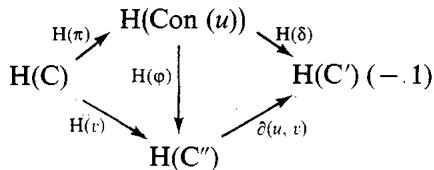
\includegraphics[keepaspectratio]{images/part001_82ee8f27.jpg}}

是可交换的，且H(φ)是双射。

在交换图（10）中，我们有 \(\mathrm{H}(1_{\mathbf{C}^{\prime}})\circ \partial (\tilde{u},\tilde{\pi}) = \partial (u,v)\circ \mathrm{H}(\varphi)\) （X，第31页，命题2）和 \(\partial (\tilde{u},\tilde{\pi}) = \mathrm{H}(\delta)\) （X，第38页，引理3，b）），因此

\[
\partial (u, v) \circ \mathbf {H} (\varphi) = \mathbf {H} (\delta);
\]

另一方面， \(\mathrm{H}(v) \circ \mathrm{H}(\beta) = \mathrm{H}(\varphi) \circ \mathrm{H}(\tilde{\pi}) = \mathrm{H}(\varphi) \circ \mathrm{H}(\pi) \circ \mathrm{H}(\beta)\) 根据X，第39页，注记。由于 \(\mathrm{H}(\beta)\) 是双射的，这给出 \(\mathrm{H}(v) = \mathrm{H}(\varphi) \circ \mathrm{H}(\pi)\) .

我们因此有 \(\partial(u, v) = H(\delta) \circ H(\varphi)^{-1}\) ，它为连接同态 \(\partial(u, v)\) 提供了一个新的定义。我们还注意到，如果把 \(H(Con(u))\) 与 \(H(C'')\) 借助 \(H(\varphi)\) 等同起来，则前面的推论表明，正合列（8）此时等同于相对于（9）的同调正合列。

\subsection{欧拉–庞加莱示性数}

在本节中，我们考虑一个由A-模的类组成的集合C，它是可加的且左正合的，即满足以下两个条件：

\begin{enumerate}
\def\labelenumi{(\Alph{enumi})}
\item
  若M和N是两个属于类型C的A-模，则M ⊕ N属于类型C。
\item
  若 \(0 \to \mathbf{M}' \to \mathbf{M} \to \mathbf{M}'' \to 0\) 是 A-模的一个正合列，且若 \(\mathbf{M}\) 与 \(\mathbf{M}''\) 属于类型 \(\mathcal{C}\) ，则 \(\mathbf{M}'\) 属于类型 \(\mathcal{C}\) .
\end{enumerate}

我们说 \(\mathcal{C}\) 是稳定的，如果它满足以下条件，这些条件蕴含(A)和(G)：

\begin{enumerate}
\def\labelenumi{(\Alph{enumi})}
\setcounter{enumi}{4}
\item
  （“C 在扩张下稳定。”）若 0 → M' → M → M'' → 0 是 A-模的短正合列，且 M' 与 M'' 属于 C 型，则 M 也属于 C 型。
\item
  （“C 在核与余核下稳定。”）对于类型 C 的 A-模的每个同态 f，A-模 Ker f 和 Coker f 均为类型 C。
\end{enumerate}

我们用 K( \(\mathcal{C}\) ) 表示 \(\mathcal{C}\) 的格罗滕迪克群，用 {[}M{]} \(_{\mathcal{C}}\) 或 {[}M{]} 表示由 A-模 M 定义的 K( \(\mathcal{C}\) ) 的元素（VIII，§ 6，第 2 节）。设 G 是一个交换群， \(\varphi\) 是从 K( \(\mathcal{C}\) ) 到 G 中的一个同态。

例子. --- 1) 若 A 是一个域，可取 C 为有限维向量空间的类组成的集合，并取 φ 为 K(C) 到 Z 上的同构，由 φ({[}M{]}) = dim (M) 定义。

\begin{enumerate}
\def\labelenumi{\arabic{enumi})}
\setcounter{enumi}{1}
\tightlist
\item
  可取 \(\mathcal{C}\) 为有限长度模的类构成的集合，并取 \(\varphi: \mathbf{K}(\mathcal{C}) \to \mathbf{Z}\) 为由 \(\varphi([\mathbf{M}]) = \text{long}_{\mathbf{A}}(\mathbf{M})\) 定义的同态。
\end{enumerate}

称分次A-模M为C型的，如果 \(M_{n}\) 对每个 n 而言都是 C 型的（为此，若 M 有界，则这是必要的；若 C 是稳定的，则这是充分的，即模 M 为 C 型）。

定义 8. --- 设 M 为一个 C 型的有界分次 A-模，并设 (M \(_{n}\) ) 为其分次。称 ∑ (-1) \(^{n}\) φ({[}M \(_{n}\) {]}) （G 的元素）为 M 的 φ-示性数，记作 χφ(M) 或简记为 χ(M)。

该定义特别适用于 M 是 A-模复形的底层分次模的情形。

例子. --- 3) 若 M 是 C 型有界的，则对每个 \(p \in Z\) ，M(p) 亦然，并且我们有 \(\chi(\mathbf{M}(p)) = (-1)^{p} \chi(\mathbf{M})\) .

\begin{enumerate}
\def\labelenumi{\arabic{enumi})}
\setcounter{enumi}{3}
\tightlist
\item
  设 \(0 \to \mathbf{M}' \to \mathbf{M} \to \mathbf{M}'' \to 0\) 是分次 A-模与次数为 0 的分次同态的一个正合列。若 \(\mathbf{M}, \mathbf{M}'\) 与 \(\mathbf{M}''\) 是 \(\mathcal{C}\) 型有界的，则我们有
\end{enumerate}

\[
\chi (\mathbf {M}) = \chi (\mathbf {M} ^ {\prime}) + \chi (\mathbf {M} ^ {\prime \prime}).
\]

如果 M 和 M'' 是类型 C 有界的，则 M' 亦然；如果 C 是稳定的，且三个模中有两个是类型 C 有界的，则第三个亦然。

\begin{enumerate}
\def\labelenumi{\arabic{enumi})}
\setcounter{enumi}{4}
\tightlist
\item
  设 \(u: \mathbf{C}' \to \mathbf{C}\) 是 \(\mathcal{C}\) 型有界复形的一个态射。则 Con \((u)\) 是 \(\mathcal{C}\) 型有界的，并且我们有：
\end{enumerate}

\[
\chi (\operatorname{Con} (u)) = \chi (\mathbf {C}) - \chi (\mathbf {C} ^ {\prime}).
\]

\begin{enumerate}
\def\labelenumi{\arabic{enumi})}
\setcounter{enumi}{5}
\tightlist
\item
  可将 G 取为群 K(C) 本身，并取 φ 为恒等映射；此时我们用 \(\chi_{\mathcal{C}}(\mathrm{M})\) 表示 K(C) 的元素 \(\chi_{\varphi}(\mathrm{M}) = \sum (-1)^{n}[\mathrm{M}_{n}]\) 。
\end{enumerate}

注记。--- 称相对于 \(\varphi\) 的元素 \(\mathrm{P}_{\mathbf{M}}(t) = \sum \varphi([\mathrm{M}_{n}]) t^{n} \in \mathrm{G} \otimes \mathbf{Z}[t, t^{-1}]\) 为 M 的庞加莱多项式。我们有 \(\mathrm{P}_{\mathbf{M}}(1) = \varphi([\mathrm{M}])\) 与 \(\mathrm{P}_{\mathbf{M}}(-1) = \chi(\mathrm{M})\) .

引理4. --- 设C是一个有界复形，类型为 \(\mathcal{C}\) 。如果 H(C) = 0，我们有 \(\chi(\mathbf{C}) = 0\) 这由第八卷，第6节，第1号，命题1的推论得出。

命题10. --- 设 C 和 C' 是两个 C 型有界复形。若存在一个拟同构 \(u: \mathbf{C}' \to \mathbf{C}\) ，则我们有 \(\chi(\mathbf{C}) = \chi(\mathbf{C}')\) .

确实，Con \((u)\) 是 \(\mathcal{C}\) 型有界的，并且我们有 \(\chi(\text{Con } (u)) = \chi(\text{C}) - \chi(\text{C}')\) ；另一方面，由 X，第 38 页，推论，H(Con \((u)) = 0\) ，因此 \(\chi(\text{Con } (u)) = 0\) （引理4）。

命题11. --- 设C是一个有界C型复形。

\begin{enumerate}
\def\labelenumi{\alph{enumi})}
\item
  若 \(\mathcal{C}\) 是稳定的，则 H(C) 是 \(\mathcal{C}\) 型的 .
\item
  如果 H(C) 是类型 C，那么 B(C) 和 Z(C) 也是，并且我们有 \(\chi(\mathrm{H}(\mathrm{C})) = \chi(\mathrm{C})\) .
\item
  若 \(\mathcal{C}\) 是稳定的，则对每个 \(n\) ，模 \(\mathbf{Z}_n(\mathbf{C})\) 是 \(\mathcal{C}\) 型的，作为 \(d_n: \mathbf{C}_n \to \mathbf{C}_{n-1}\) 的核；且 \(\mathrm{H}_n(\mathbf{C})\) 是 \(\mathcal{C}\) 型的，作为 \(\mathbf{C}_{n+1} \to \mathbf{Z}_n\) 的余核。另一方面， \(\mathrm{H}_n(\mathbf{C}) = 0\) （只要 \(\mathbf{C}_n = 0\) ）.
\item
  假设 H(C) 是 C 型的。典范正合列：
\end{enumerate}

\[
0 \to Z _ {n} (\mathbf {C}) \to C _ {n} \to B _ {n - 1} (\mathbf {C}) \to 0
\]

\[
0 \to \mathrm{B} _ {n} (\mathrm{C}) \to \mathrm{Z} _ {n} (\mathrm{C}) \to \mathrm{H} _ {n} (\mathrm{C}) \to 0
\]

从 C 的右界出发对 n 作归纳可知， \(Z_{n}(C)\) 与 \(B_{n}(C)\) 对每个 n 都是 C 型的。于是我们有

\[
\chi (\mathrm{C}) = \chi (\mathrm{Z} (\mathrm{C})) + \chi (\mathrm{B} (\mathrm{C}) (- 1)) = \chi (\mathrm{Z} (\mathrm{C})) - \chi (\mathrm{B} (\mathrm{C})) = \chi (\mathrm{H} (\mathrm{C})).
\]

推论。 --- 若 C 是稳定的且 C 是 C 型有界的，则分次模 H(C) 是 C 型有界的，并且我们有 \(\chi(\mathrm{H}(\mathrm{C})) = \chi(\mathrm{C})\) .

命题12. --- 设 \(0 \to C' \to C \to C'' \to 0\) 是复形的一个正合列。a) 若 H(C)、H(C') 和 H(C'') 是 C 型有界的，则我们有

\[
\chi (\mathrm{H} (\mathbf {C})) = \chi (\mathrm{H} (\mathbf {C} ^ {\prime})) + \chi (\mathrm{H} (\mathbf {C} ^ {\prime \prime})) .
\]

\begin{enumerate}
\def\labelenumi{\alph{enumi})}
\setcounter{enumi}{1}
\tightlist
\item
  如果C是稳定的，并且分次模H(C)、H(C')和H(C'')中有两个是C型有界的，那么第三个也是。
\end{enumerate}

a) 由将引理4应用于由所给正合列相关联的同调正合列所定义的零同调复形得出。b) 通过考虑该同调正合列，由以下引理得出：

引理5. --- 设 M → N → P → Q → R 是 A-模的正合列。若 C 是稳定的，且 M、N、Q 和 R 属于 C 型，则模 P 属于 C 型。

令 \(\mathbf{N}' = \operatorname{Coker} (\mathbf{M} \to \mathbf{N})\) 与 \(\mathbf{Q}' = \operatorname{Ker} (\mathbf{Q} \to \mathbf{R})\) 。模 \(\mathbf{N}'\) 与 \(\mathbf{Q}'\) 属于类型 \(\mathcal{C}\) ，并且我们有一个正合列 \(0 \to \mathbf{N}' \to \mathbf{P} \to \mathbf{Q}' \to 0\) .

推论。--- 假设 C 是稳定的，并设 \(u : C' \to C\) 是复形的一个态射，使得 \(\mathrm{H}(\mathbf{C})\) 与 \(\mathrm{H}(\mathbf{C}')\) 是 C 型有界的。则 \(\mathrm{H}(\mathrm{Con}(u))\) 是 C 型有界的，并且我们有

\[
\chi (\mathrm{H} (\text { Con } (u))) = \chi (\mathrm{H} (\mathrm{C})) - \chi (\mathrm{H} (\mathrm{C} ^ {\prime})) .
\]

这由命题 12 应用于复形的正合列（X，第 37 页，命题 7）得出

\[
0 \rightarrow \mathrm{C} \rightarrow \operatorname{Con} (u) \rightarrow \mathrm{C} ^ {\prime} (- 1) \rightarrow 0.
\]

注记。--- 设 E 是一个复形， \(h: \mathrm{E} \to \mathrm{C}\) 与 \(h': \mathrm{E} \to \mathrm{C}'\) 是同伦等价，其中 C 与 C' 是 \(\mathcal{C}\) 型有界的。则我们有 \(\chi(\mathrm{C}) = \chi(\mathrm{C}')\) 。事实上，若 \(h_1\) 是 \(h\) 在同伦意义下的逆，则 \(h' \circ h_1\) 是一个同伦等价，因此是从 C 到

C' 的一个拟同构，从而可以应用命题10。因此，只要存在从 E 到 C 型有界复形 C 的同伦等价，就可以通过设定 \(\chi(E) = \chi(C)\) 来扩展定义 8。命题 10、11、12 及其推论均可推广到这一情形。

应用：

* 设 X 是一个容许有限胞腔分解的拓扑空间（参见第 3 节）。a) 设 K 和 K' 是两个域，令 \(b_i = \dim_K(\mathrm{H}_i(\mathrm{X}, \mathrm{K}))\) 与 \(b_i' = \dim_K(\mathrm{H}_i(\mathrm{X}, \mathrm{K}'))\) 。我们不一定有 \(b_i = b_i'\) ，但有 \(\Sigma(-1)^i b_i = \Sigma(-1)^i b_i'\) .

\begin{enumerate}
\def\labelenumi{\alph{enumi})}
\setcounter{enumi}{1}
\tightlist
\item
  设 \((\mathbf{X}_{n})\) 与 \((\mathbf{X}_{n}^{\prime})\) 是 X 的两个有限胞腔分解，并设 \(c_{n}\) 与 \(c_{n}^{\prime}\) 是这两个分解中 n 维胞腔的个数。我们有
\end{enumerate}

\[
\Sigma (- 1) ^ {i} c _ {i} = \Sigma (- 1) ^ {i} c _ {i} ^ {\prime}.
\]

\begin{enumerate}
\def\labelenumi{\alph{enumi})}
\setcounter{enumi}{2}
\tightlist
\item
  利用 \(a)\) 与 \(b)\) 的记号，我们有 \(\Sigma(-1)^{i} c_{i} = \Sigma(-1)^{i} b_{i}\) .
\end{enumerate}

性质 \(a\) ) 与 \(b\) ) 由 \(c\) ) 推出，而 \(c\) ) 由命题11应用于第 3 号中所述的复形 \(\Gamma\) 得出，取 \(\mathscr{C}\) 为有限维 K-向量空间的类，取 \(\varphi\) 为由 \(\varphi([\mathrm{M}]) = \dim_{\mathrm{K}}(\mathrm{M})\) 定义的函数（X，第 40 页，例 1）。*

\subsection{右模复形，多模复形}

右A-模的复形是一个分次右A-模 \((M_{n})_{n\in\mathbf{Z}}\) 配备了一个次数为-1且平方为零的分次自同态；因此它是环A°（与A相反）上的模复形。因此，前面各节所述的所有定义和性质都适用于右模复形，这些右模复形被视为环A°上的模复形。

类似地，若 A 和 B 是两个环，则 (A, B)-双模复形是配备有一个分次自同态 \(d\) （次数为 \((-1)\) 且平方为零）的分次 (A, B)-双模 M；若赋予 M 其作为左 A \(\otimes_{\mathbf{z}} \mathbf{B}^{\circ}\) -模的典范结构，则 \(d\) 赋予它一个 A \(\otimes_{\mathbf{z}} \mathbf{B}^{\circ}\) -复形的结构。因此，前面各节中陈述的所有定义和性质均适用于双模复形。多模复形的定义类似。

\subsection{例子：德拉姆复形}

在本节中，我们假设 A 是交换环 \(k\) 上的一个交换 \(k\) -代数。用 \(\Omega_{\mathbf{A}/k}^{1}\) 表示 A 的凯勒微分 A-模（III，第 134 页），用 \(d^{0}: \mathbf{A} \to \Omega_{\mathbf{A}/k}^{1}\) 表示 \(k\) -导子 \(d_{\mathbf{A}/k}\) ，并用 \(\Omega_{\mathbf{A}/k}\) 表示分次 \(k\) -代数 \(\boldsymbol{\Lambda}_{\mathbf{A}}(\Omega_{\mathbf{A}/k}^{1})\) .

命题13. --- 存在唯一的次数为 1、平方为零的 k-反导子 \(d: \Omega_{\mathbf{A}/k} \to \Omega_{\mathbf{A}/k}\) ，它延拓导子 \(d^{0}: \mathbf{A} \to \Omega_{\mathbf{A}/k}^{1}\) .

让我们证明反导子 \(d\) 的唯一性。由于 \(d \circ d = 0\) ，我们有，对于 \(y, x_1, \ldots, x_p \in \mathbf{A}\) :

\[
d \left(y d x _ {1} \wedge \dots \wedge d x _ {p}\right) = d y \wedge d x _ {1} \wedge \dots \wedge d x _ {p}.
\]

A-模 \(\Omega_{\mathbf{A}/k}^{p}\) 由元素 \(dx_{1} \wedge \ldots \wedge dx_{p}\) 生成，这就证明了 \(d\) 的唯一性 .

为了证明存在性，只需构造一个 \(k\) -同态 \(d^{1}:\Omega_{\mathbb{A}/k}^{1}\to\Omega_{\mathbb{A}/k}^{2}\) ，使得 \(d^{1}\circ d^{0}=0\) 且

\[
d ^ {1} (a \omega) = d ^ {0} (a) \wedge \omega + a d ^ {1} (\omega) \quad \text {for} \quad a \in A, \quad \omega \in \Omega_ {A k} ^ {1}.\tag{11}
\]

事实上，由 III，第 128 页，命题 14（考虑到 III，第 118 页，注记 2）可知，存在一个反导子 \(d: \Omega_{\mathbf{A}/k} \to \Omega_{\mathbf{A}/k}\) ，它在次数为 0 时与 \(d^{0}\) 重合，在次数为 1 时与 \(d^{1}\) 重合。由于 \(d^{0}\) 在 \(\mathbf{A}\) 上为零，反导子 \(d\) 是 \(k\) -线性的；由于 \(d^{1} \circ d^{0} = 0\) ，我们有 \(d \circ d = 0\) ，因为 \(\Omega_{\mathbf{A}/k}\) 作为 \(\mathbf{A}\) -代数由元素 \(d^{0} a\) （ \(a \in \mathbf{A}\) ）生成 .

为了定义 \(d^{1}\) ，回顾（III，第 133 页） \(\Omega_{\mathbf{A}/k}^{1}\) 等于 A-模 \(\mathfrak{I}/\mathfrak{I}^{2}\) ，其中 \(\mathfrak{I}\) 是乘法 \(m: \mathbf{A} \otimes_{k} \mathbf{A} \to \mathbf{A}\) 的核。考虑 \(k\) -线性映射 \(u: \mathbf{A} \otimes_{k} \mathbf{A} \to \Omega_{\mathbf{A}/k}^{2}\) ，它由 \(u(x \otimes y) = d^{0}(y) \wedge d^{0}(x)\) 定义。我们有

\[
u (a x \otimes y - x \otimes a y) = d ^ {0} (y) \wedge d ^ {0} (a x) - d ^ {0} (a y) \wedge d ^ {0} (x) = d ^ {0} (x y) \wedge d ^ {0} (a)
\]

对于 A 中的 x、y 和 a，由此可得

\[
u ((a \otimes 1 - 1 \otimes a) \xi) = d ^ {0} (m (\xi)) \wedge d ^ {0} (a), \quad \xi \in \mathrm{A} \otimes_ {k} \mathrm{A}, \quad a \in \mathrm{A}. \tag {12}
\]

由于 \(\mathfrak{I}\) 作为左 A-模由元素 ( \(a \otimes 1 - 1 \otimes a\) ) （ \(a \in \mathbf{A}\) ）生成，我们推出 \(u(\mathfrak{I}^2) = 0\) ；因此 \(u\) 通过限制到 \(\mathfrak{I}\) 并过渡到商，定义了一个 \(k\) -线性映射 \(d^1: \mathfrak{I}/\mathfrak{I}^2 \to \Omega_{\mathrm{A}/k}^2\) .

在（12）中取 \(\xi = b \otimes 1\) （其中 \(b \in \mathbf{A}\) ），我们得到 \(d^{1}(bd^{0}(a)) = d^{0}(b) \wedge d^{0}(a)\) ；由此得出 \(d^{1} \circ d^{0} = 0\) ，以及 \(d^{1}(c\omega) = d^{0}(c) \wedge \omega + cd^{1}(\omega)\) （对 \(c \in \mathbf{A}\) 与 \(\omega = bd^{0}(a)\) ）。由于 \(\Omega_{\mathbf{A}/k}^{1}\) 作为 \(k\) -模由元素 \(bd^{0}(a)\) （ \(a\) 与 \(b\) 属于 \(\mathbf{A}\) ）生成，公式（11）对所有 \(\omega \in \Omega_{\mathbf{A}/k}\) 成立，这就完成了命题的证明。

有时称元素 \(\omega\in\Omega_{A/k}^{p}\) 为次数为 \(p\) 的外微分形式（A 在 \(k\) 上），并称反导子 \(d\) 为 \(\Omega_{A/k}\) 的外微分；复形（ \(\Omega_{A/k}\) , \(d\) ）称为 A 在 \(k\) 上的德拉姆复形，其同调为 A 在 \(k\) 上的德拉姆上同调 .

例 1. --- 取 A 为环 \(k[\mathbf{X}_{1},\ldots,\mathbf{X}_{n}]\) 。则 \(\Omega_{\mathbf{A}/k}^{1}\) 是一个自由 A-模，其基为 \(d\mathbf{X}_{1},\ldots,d\mathbf{X}_{n}\) （III，第 134 页，例）。因此，若对每个子集 \(\mathrm{I}=\{i_{1},\ldots,i_{p}\}\) （ \([1,n]\) 的）设 \(d\mathbf{X}_{\mathrm{I}}=d\mathbf{X}_{i_{1}}\wedge\ldots\wedge d\mathbf{X}_{i_{p}}\) （其中 \(i_{1}<\ldots<i_{p}\) ），则 A-模 \(\Omega_{\mathbf{A}/k}^{p}\) 以元素 \(d\mathbf{X}_{\mathrm{I}}\) 为基，其中 I 遍历 \([1,n]\) 的基数为 \(p\) 的子集的集合。我们有

\[
d (\mathrm{P} d \mathrm{X} _ {\mathrm{I}}) = d \mathrm{P} \wedge d \mathrm{X} _ {\mathrm{I}} = \sum_ {i \notin \mathrm{I}} (- 1) ^ {n (\mathrm{I}, i)} \frac {\partial \mathrm{P}}{\partial \mathrm{X} _ {i}} d \mathrm{X} _ {\mathrm{I} \cup \{i \}},
\]

其中 \(n(\mathbf{I}, i)\) 表示 I 中严格小于 \(i\) 的元素的个数 .

\(Z^{p}(\Omega_{\mathbf{A}/k})\) 的闭链因此是这样的元素 \(\omega = \sum_{\text{Card (I)} = p} \mathrm{P}_{\mathrm{I}} d\mathrm{X}_{\mathrm{I}}\) ：对每个子集 \(J\) （含 \((p + 1)\) 个元素，属于 \([1, n]\) ），有：

\[
\sum_ {i \in J} (- 1) ^ {n (J, i)} \frac {\partial P _ {J - \{i \}}}{\partial X _ {i}} = 0.
\]

元素 ω 是一个边缘，如果对于每个子集 \(J \subset [1, n]\) （含 \((p - 1)\) 个元素），可以选择一个多项式 \(Q_{J} \in A\) ，使得：

\[
\mathrm{P} _ {\mathrm{I}} = \sum_ {j \in \mathrm{I}} (- 1) ^ {n (\mathrm{I}, j)} \frac {\partial \mathrm{Q} _ {\mathrm{I} - \{j \}}}{\partial \mathrm{X} _ {j}}.
\]

我们将在 § 9 中看到，如果 k 是一个 Q-代数，则 A 在 k 上的德拉姆复形在次数 \textgreater{} 0 上是零调的（X，第 159 页，注记 4）。

* 例 2. --- 假设 \(k = \mathbf{C}\) 且 \(\mathbf{A} = \mathbf{C}\) \([\mathrm{X}_1, \ldots, \mathrm{X}_n] / (\mathrm{P}_1, \ldots, \mathrm{P}_r)\) ，其中 \(\mathrm{P}_i\) 是 \(\mathrm{X}_1, \ldots, \mathrm{X}_n\) 的多项式，使得 \(\mathbf{C}^n\) 中所有 \(\mathrm{P}_i\) 为零的点集是 \(\mathbf{C}^n\) 的一个解析子流形 V。可以证明 A 在 C 上的德拉姆上拟同构于奇异上同调 H(V, C)。*

设 M 是一个 A-模，且 \(\nabla^{0}\) 为 \(k\) -线性映射，从 M 到 \(\mathbf{M} \otimes_{\mathbf{A}} \Omega_{\mathbf{A}/k}^{1}\) 使得

\[
\nabla^ {0} (a m) = a \nabla^ {0} (m) + m \otimes d a \quad \text { for } \quad a \in \mathrm{A}, \quad m \in \mathrm{M}\tag{13}
\]

（有时也称 \(\nabla^{0}\) 为 A-模 M 上的一个联络）。

命题 14. --- (i) 存在唯一的 k-线性映射 \(\nabla\) 从 \(\Omega_{\mathbf{A}/k}\) 右模 \(\mathbf{M} \otimes_{\mathbf{A}} \Omega_{\mathbf{A}/k}\) 到自身，次数为 1 的分次映射，它扩展了 \(\nabla^{0}\) 在次数0中，并满足恒等式：

\[
\nabla (x \omega) = (\nabla x) \omega + (- 1) ^ {p} x (d \omega) \quad \mathrm{for} \quad x \in \mathrm{M} \otimes_ {\mathrm{A}} \Omega_ {\mathrm{A} / k} ^ {p}, \quad \omega \in \Omega_ {\mathrm{A} / k}. \tag {14}
\]

\begin{enumerate}
\def\labelenumi{(\roman{enumi})}
\setcounter{enumi}{1}
\tightlist
\item
  复合映射 \(\nabla \circ \nabla\) 是 \(\Omega_{\mathbf{A} / k}\) -线性；特别地，映射 \(\mathbf{R} = \nabla^{1} \circ \nabla^{0}\) 的 \(\mathbf{M}\) 到 \(\mathbf{M} \otimes_{\mathbf{A}} \Omega_{\mathbf{A} / k}^{2}\) 是 \(\mathbf{A}\) -线性，并且我们有
\end{enumerate}

\[
\nabla \circ \nabla (m \otimes \omega) = R (m). \omega \quad \mathrm{for} \quad m \in M, \quad \omega \in \Omega_ {A / k}.
\]

同态 R 有时称为联络 \(\nabla^{0}\) 的曲率同态；若它为零，则偶对 \((\mathbf{M} \otimes_{\mathbf{A}} \Omega_{\mathbf{A}/k}, \nabla)\) 是一个复形，也称为 \((\mathbf{M}, \nabla^{0})\) 在 \(k\) 上的德拉姆复形 .

我们来证明 (i)。 \(\nabla\) 的唯一性是显然的。让我们定义一个 \(k\) -同态 \(\overline{\nabla}\) ，从 \(\mathbf{M} \otimes_k \Omega_{\mathbf{A}/k}\) 到 \(\mathbf{M} \otimes_{\mathbf{A}} \Omega_{\mathbf{A}/k}\) ：

\[
\overline {{{\nabla}}} (m \otimes_ {k} \omega) = (\nabla^ {0} m) \omega + m \otimes d \omega \quad \text { for } \quad m \in \mathbf {M}, \quad \omega \in \Omega_ {\mathrm{A} / k}.
\]

由（13）可得 \(\overline{\nabla}(am \otimes \omega) = \overline{\nabla}(m \otimes a\omega)\) ，因此通过过渡到商，我们得到一个 \(k\) -同态 \(\nabla\) ，它从 \(\mathbf{M} \otimes_{\mathbf{A}} \Omega_{\mathbf{A}/k}\) 到自身、次数为 1 的分次映射，且在次数 0 时延拓 \(\nabla^{0}\) 。让我们验证（14）：我们有，对于 \(m \in \mathbf{M}\) , \(\alpha \in \Omega_{\mathbf{A}/k}^{p}\) , \(\omega \in \Omega_{\mathbf{A}/k}\) :

\[
\begin{array}{r l} \nabla ((m \otimes \alpha). \omega) & = \nabla (m \otimes (\alpha \wedge \omega)) = \nabla^ {0} (m). (\alpha \wedge \omega) + m \otimes d (\alpha \wedge \omega) \\ & = \nabla^ {0} (m) \alpha . \omega + (m \otimes d \alpha) \omega + (- 1) ^ {p} (m \otimes \alpha) d \omega \\ & = (\nabla (m \otimes \alpha)) \omega + (- 1) ^ {p} (m \otimes \alpha) d \omega \end{array}
\]

这证明了 (14) 式对 \(x = m \otimes \alpha\) 成立；一般情形由此通过线性性推出。

让我们证明(ii)。设 \(x \in \mathbf{M} \otimes_{\mathbf{A}} \Omega_{\mathbf{A}/k}^{p}\) , \(\omega \in \Omega_{\mathbf{A}/k}\) ；通过反复应用(14)，我们得到：

\[
\begin{array}{r l} \nabla \circ \nabla (x \omega) = & \nabla (\nabla (x) \omega) + (- 1) ^ {p} \nabla (x d \omega) \\ & = (\nabla \circ \nabla (x)) \omega + (- 1) ^ {p + 1} \nabla (x) (d \omega) + (- 1) ^ {p} \nabla (x) (d \omega) \\ & = (\nabla \circ \nabla (x)) \omega , \end{array}
\]

这证明了(ii)的第一个断言；其余断言随之立即成立。

\section{分解}

我们沿用上一节的约定。

\subsection{复形态射的扩张}

引理1. --- 考虑一个由A-模及同态构成的图表

\[
\begin{array}{c} \mathbf {M} ^ {\prime} \xrightarrow {\alpha^ {\prime}} \mathbf {M} \xrightarrow {\alpha} \mathbf {M} ^ {\prime \prime} \\ f ^ {\prime} \Biggl \downarrow \quad \swarrow k / f \Biggl \downarrow \quad \swarrow k ^ {\prime \prime} \\ \mathbf {N} ^ {\prime} \xrightarrow [ \beta^ {\prime} ]{} \mathbf {N} \xrightarrow [ \beta ]{} \mathbf {N} ^ {\prime \prime} \end{array}
\]

使得 \(f \circ \alpha' = \beta \circ f', \alpha \circ \alpha' = 0\) ，Ker \(\beta = \operatorname{Im} \beta'\) ，且 \(f = k'' \circ \alpha + \beta \circ k\) 且其中 \(\mathbf{M}'\) 是投射的。存在一个A-同态 \(k': \mathbf{M}' \to \mathbf{N}'\) 使得 \(f' = k \circ \alpha' + \beta' \circ k'\) .

事实上，令 \(g = f' - k \circ \alpha'\) ；我们有

\[
\beta \circ g = \beta \circ f ^ {\prime} - \beta \circ k \circ \alpha^ {\prime} = f \circ \alpha^ {\prime} - \beta \circ k \circ \alpha^ {\prime} = k ^ {\prime \prime} \circ \alpha \circ \alpha^ {\prime} = 0.
\]

这意味着 \(\operatorname{Im}(g) \subset \operatorname{Ker}(\beta) = \operatorname{Im}(\beta')\) 。由于 \(\mathbf{M}'\) 是投射的，因此存在一个A-同态 \(k': \mathbf{M}' \to \mathbf{N}'\) 使得 \(\beta' \circ k' = g\) ，从而引理得证。

引理2. --- 如果在A-模与同态的交换图中

\[
\begin{array}{c c c c c} \mathbf {M} ^ {\prime} & \xrightarrow {\alpha^ {\prime}} & \mathbf {M} & \xrightarrow {\alpha} & \mathbf {M} ^ {\prime \prime} \\ & & \Big \downarrow^ {u} & & \Big \downarrow^ {u ^ {\prime \prime}} \\ \mathbf {N} ^ {\prime} & \xrightarrow {\beta^ {\prime}} & \mathbf {N} & \xrightarrow {\beta} & \mathbf {N} ^ {\prime \prime} \end{array}
\]

我们有 \(\alpha\circ\alpha'\) =0，Ker \(\beta=\operatorname{Im}\beta'\) 且如果 \(\mathbf{M}'\) 是投射的，则存在一个A-同态 \(u':\mathbf{M}'\to\mathbf{N}'\) 使得 \(\beta'\circ u'=u\circ\alpha'\) .

只需在引理1中设 \(k'' = u'', k = -u, f = 0, f' = 0\) 与 \(u' = k'\) 即可。

引理1 bis. --- 考虑一个A-模与同态的图表

\[
\begin{array}{c} \mathbf {M} ^ {\prime} \xrightarrow {\alpha^ {\prime}} \mathbf {M} \xrightarrow {\alpha} \mathbf {M} ^ {\prime \prime} \\ \Big \downarrow_ {k ^ {\prime}} \Big \downarrow_ {f ^ {\prime}} \Big \downarrow_ {k} \Big \downarrow_ {f} \\ \mathbf {N} ^ {\prime} \xrightarrow [ \beta^ {\prime} ]{} \mathbf {N} \xrightarrow [ \beta ]{} \mathbf {N} ^ {\prime \prime} \end{array}
\]

使得 \(f \circ \alpha' = \beta \circ f'\) ，Ker \(\alpha = \operatorname{Im} \alpha'\) , \(\beta \circ \beta' = 0\) ，且 \(f' = k \circ \alpha' + \beta' \circ k'\) ，且其中 \(N''\) 是单射的。存在一个 A-同态 \(k'' : M'' \to N''\) 使得 \(f = k'' \circ \alpha + \beta \circ k\) 。事实上，设 \(q = f - \beta \circ k\) ，我们有

\[
g \circ \alpha^ {\prime} = f \circ \alpha^ {\prime} - \beta \circ k \circ \alpha^ {\prime} = \beta \circ f ^ {\prime} - \beta \circ k \circ \alpha^ {\prime} = \beta \circ \beta^ {\prime} \circ k ^ {\prime} = 0.
\]

这蕴含Ker \(g \supset \operatorname{Im} \alpha' = \operatorname{Ker} \alpha\) 。由于 \(\mathbf{N}''\) 是单射的，因此（X，第16页，注记）存在一个A-同态 \(k': \mathbf{M}'' \to \mathbf{N}''\) 使得 \(g = k'' \circ \alpha\) ，从而引理得证。

引理2 bis. --- 若在A-模与同态的交换图中

\[
\begin{array}{c c c c c} \mathbf {M} ^ {\prime} & \stackrel {{\alpha^ {\prime}}} {{\longrightarrow}} & \mathbf {M} & \stackrel {{\alpha}} {{\longrightarrow}} & \mathbf {M} ^ {\prime \prime} \\ u ^ {\prime} \Big \downarrow & & u \Big \downarrow & & \\ \mathbf {N} ^ {\prime} & \stackrel {{\beta^ {\prime}}} {{\longrightarrow}} & \mathbf {N} & \stackrel {{\beta}} {{\longrightarrow}} & \mathbf {N} ^ {\prime \prime}, \end{array}
\]

我们有 \(\operatorname{Ker} \alpha = \operatorname{Im} \alpha'\) , \(\beta \circ \beta' = 0\) 且如果 \(\mathbf{N}''\) 是单射的，则存在一个A-同态 \(u'' : \mathbf{M}'' \to \mathbf{N}''\) 使得 \(u'' \circ \alpha = \beta \circ u\) .

只需在引理 1 bis 中设 \(u' = k', u = -k, f = 0, f' = 0\) 与 \(k'' = u''\) 即可。

命题1. --- 设(P, \(d_{\mathbb{P}}\) ) 和 (E, \(d_{\mathbb{E}}\) ) 是 A-模的两个复形，且 r 是一个整数。

\begin{enumerate}
\def\labelenumi{\alph{enumi})}
\item
  设 \((u_i: \mathrm{P}_i \to \mathrm{E}_i)_{i \leqslant r}\) 是一个同态族，使得 \(d_{\mathrm{E}} \circ u_i = u_{i-1} \circ d_P\) （对 \(i \leqslant r\) ）。假设 \(\mathrm{P}_i\) 对 \(i > r\) 是投射的，且 \(\mathrm{H}_i(\mathrm{E}) = 0\) （对 \(i \geqslant r\) ）。则 \(u_i\) 的族可延拓为从 P 到 E 的一个复形态射；两个这样的延拓是同伦的。
\item
  设 \((u^{i}:\mathbf{P}^{i}\to\mathbf{E}^{i})_{i\leqslant r}\) 是一个同态族，使得 \(u^{i}\circ d_{\mathrm{P}}=d_{\mathrm{E}}\circ u^{i-1}\) （对 \(i\leqslant r\) ）。假设 \(\mathbf{E}^{i}\) 对 \(i>r\) 是单射的，且 \(\mathbf{H}^{i}(\mathbf{P})=0\) （对 \(i\geqslant r\) ）。则 \(u^{i}\) 的族可延拓为从 \(\mathbf{P}\) 到 \(\mathbf{E}\) 的一个复形态射；两个这样的延拓是同伦的。
\end{enumerate}

让我们证明 a)。族 \((u_{i})_{i\leqslant r}\) 的一个扩张 v 的存在性由引理 2 通过归纳法直接得出。设 \(v'\) 是另一个扩张；设 \(f=v'-v\) ，并对整数 n 作归纳，构造一个同态 \(k_{n}:P_{n}\to E_{n+1}\) ，使得 \(f_{n}=d_{E}\circ k_{n}+k_{n-1}\circ d_{P}\) 。对 \(i\leqslant r\) ，取 \(k_{i}=0\) 。设 \(n\geqslant r\) 并假设 \(k_{i}\) 对 \(i\leqslant n\) 已构造。于是考虑图表

\[
\begin{array}{c} \mathrm{P} _ {n + 1} \xrightarrow {d _ {\mathrm{p}}} \mathrm{P} _ {n} \xrightarrow {d _ {\mathrm{p}}} \mathrm{P} _ {n - 1} \\ f _ {n + 1} \Biggl \downarrow \quad k _ {n} \Biggl \downarrow f _ {n} \Biggl \downarrow k _ {n - 1} \\ \mathrm{E} _ {n + 2} \xrightarrow {d _ {\mathrm{E}}} \mathrm{E} _ {n + 1} \xrightarrow {d _ {\mathrm{E}}} \mathrm{E} _ {n}. \end{array}
\]

引理1的假设得到满足；因此存在一个A-同态 \(k_{n+1}: \mathbf{P}_{n+1} \to \mathbf{E}_{n+2}\) 使得 \(f_{n+1} = d_{\mathbf{E}} \circ k_{n+1} + k_n \circ d_p\) ，从而 \(a\) ).

b) 的证明类似，借助引理 1 bis 与引理 2 bis 完成。

\subsection{分解}

在下文中，总是将模与一个复形等同起来，该复形以该模为零次分量，且所有其他分量为零。

定义1. --- 设 M 为一个 A-模。M 的一个左分解是一个偶对 (P, p)，其中 P 是一个在右侧为零的复形，且 p : P → M 是一个拟同构。M 的一个右分解是一个偶对 (e, E)，其中 E 是一个在左侧为零的复形，且 e : M → E 是一个拟同构。

称分解(P, p)（相应地(e, E)）的长度为复形P（相应地E）的长度。若(P, p)和(P', p')（相应地(e, E)和(e', E')）是M的两个左（相应地右）分解，则一个复形态射 \(f: P \to P'\) 使得 \(p' \circ f = p\) (相应地， \(g: E \to E'\) 使得 \(g \circ e = e'\) ）被称为分解的态射。

命题2. --- 设 P 为一个在右侧为零的复形，且设 p : P → M 为一个态射。要使 (P, p) 成为 M 的一个左分解，必要且充分条件是序列

\[
\dots \longrightarrow \mathrm{P} _ {n} \xrightarrow {d _ {\mathrm{P}}} \mathrm{P} _ {n - 1} \longrightarrow \dots \quad \longrightarrow \mathrm{P} _ {1} \xrightarrow {d _ {\mathrm{P}}} \mathrm{P} _ {0} \xrightarrow {p _ {0}} \mathrm{M} \longrightarrow 0\tag{1}
\]

是正合的。

事实上，说 \(p: \mathbf{P} \to \mathbf{M}\) 是拟同构，意味着 \(\mathrm{H}_{i}(\mathbf{P}) = 0\) （对 \(i > 0\) ），且 \(p_{0}\) 诱导了从 Coker ( \(d_{\mathbf{P}}: \mathbf{P}_{1} \to \mathbf{P}_{0}\) ) 到 \(\mathbf{M}\) 上的一个同构 .

的同构。类似地：

命题2bis. --- 设 E 是一个在左侧为零的复形，并设 e : M → E 是一个态射。要使 (e, E) 成为 M 的一个右分解，必要且充分条件是序列

\[
0 \longrightarrow \mathrm{M} \stackrel {e _ {0}} {\longrightarrow} \mathrm{E} ^ {0} \stackrel {d _ {\mathrm{E}}} {\longrightarrow} \mathrm{E} ^ {1} \longrightarrow \dots \longrightarrow \mathrm{E} ^ {n} \stackrel {d _ {\mathrm{E}}} {\longrightarrow} \mathrm{E} ^ {n + 1} \longrightarrow \dots\tag{1 bis}
\]

是正合的。

为方便起见，人们常说序列 (1)（相应地 (1 bis)）是 M 的左（相应地右）分解。

定义2. --- A-模 M 的一个投射（相应地自由、相应地平坦）分解是 M 的一个左分解 (P, p)，使得复形 P 是投射的（相应地自由的、相应地平坦的）（X，第 25 页）。M 的一个内射分解是 M 的一个右分解 (e, E)，使得复形 E 是内射的（同上）。

例子. --- 1) 假设环 A 是主理想整环；设 M 是一个 A-模，并设 \((x_{i})_{i\in I}\) 是 M 的一个生成族。设 \(L_{0}\) 是自由模 \(\mathbf{A}^{(I)}\) , \((e_{i})\) 为其典范基，并定义 \(p:L_{0}\to\mathbf{M}\) 为 \(p(e_{i})=x_{i}\) 。态射 \(p\) 是满射的，且其核 \(L_{1}\) 由 VII, § 3, 定理 1 的推论 2 知是一个自由 A-模，因此正合列

\[
0 \to \mathrm{L} _ {1} \to \mathrm{L} _ {0} \xrightarrow {p} \mathrm{M} \to 0
\]

是 M 的长度为 1 的自由分解。若 I 是有限的，则 \(L_{0}\) 与 \(L_{1}\) 是有限生成的。

\begin{enumerate}
\def\labelenumi{\arabic{enumi})}
\setcounter{enumi}{1}
\tightlist
\item
  假设 A 是交换的；设 E 是一个 A-模，u 是 E 的一个自同态。记 \(E_{u}\) 为通过赋予 E 由下式定义的结构而得到的 A{[}X{]}-模
\end{enumerate}

\[
(p, x) \mapsto p (u) (x) \quad \text { for } \quad p \in \mathrm{A} [ \mathrm{X} ] \quad \text { and } \quad x \in \mathrm{E}.
\]

根据III，第106页，我们有一个正合列：

\[
0 \to \mathrm{A} [ \mathrm{X} ] \otimes_ {\mathrm{A}} \mathrm{E} \stackrel {\psi} {\to} \mathrm{A} [ \mathrm{X} ] \otimes_ {\mathrm{A}} \mathrm{E} \stackrel {\varphi} {\to} \mathrm{E} _ {u} \to 0
\]

其中 \(\varphi(p \otimes x) = p.x\) 与 \(\psi(p \otimes x) = Xp \otimes x - p \otimes u(x)\) （当 \(p \in A[X]\) 与 \(x \in E\) ）。这个正合列是 \(E_u\) 的长度为 1 的自由（相应地，投射，相应地，有限生成）分解，如果 E 是自由（相应地，投射，相应地，有限生成）A-模。3) 如果 A 是主理想整环，则正合列

\[
0 \rightarrow \mathrm{A} \rightarrow \mathrm{K} \rightarrow \mathrm{K/A} \rightarrow 0
\]

是 A-模 \(\mathbf{A}_s\) 的长度为 1 的内射分解（X，第 18 页，例 1）。

命题 3. --- 设 \(f: \mathbf{M}' \to \mathbf{M}\) 是 A-模的一个同态， \(p': \mathbf{P}' \to \mathbf{M}'\) 是到 \(\mathbf{M}'\) 的、来自一个在右侧为零且投射的复形 \(\mathbf{P}'\) 的一个态射，且 \(p: \mathbf{P} \to \mathbf{M}\) 是 M 的一个左分解。存在一个复形态射 \(\tilde{f}: \mathbf{P}' \to \mathbf{P}\) ，且在同伦意义下唯一，使得 \(p \circ \tilde{f} = f \circ p'\) .

考虑如下定义的复形 \(\overline{\mathbf{P}}\) ： \(\overline{\mathbf{P}}_n = \mathbf{P}_n\) 当 \(n \neq -1\) , \(\overline{\mathbf{P}}_{-1} = \mathbf{M}\) , \(d_{\overline{\mathbf{P}},n} = d_{\mathbf{P},n}\) 当 \(n \neq 0, -1\) , \(d_{\overline{\mathbf{P}},0} = p_0\) , \(d_{\overline{\mathbf{P}},-1} = 0\) ，以及类似定义的复形 \(\overline{\mathbf{P}}'\) 。将命题 1 a) 应用于复形 \(\overline{\mathbf{P}}\) 与 \(\overline{\mathbf{P}}'\) ，取 \(r=0\) , \(u_i = 0\) （当 \(i < -1\) ）与 \(u_{-1} = f\) ，我们得到命题 3。

推论。--- 设 (P, p) 与 (P', p') 是 M 的两个投射分解。存在一个在同伦意义下唯一的同伦等价 \(\alpha: P' \to P\) ，使得 \(p \circ \alpha = p'\) .

事实上，存在一个态射 \(\alpha: P' \to P\) (相应地， \(\beta: P \to P'\) ）使得 \(p \circ \alpha = p'\) (相应地， \(p' \circ \beta = p\) ）。由于 \(p \circ \alpha \circ \beta = p\) (相应地， \(p' \circ \beta \circ \alpha = p'\) ), \(\alpha \circ \beta\) 同伦于 \(1_P\) (相应地， \(\beta \circ \alpha\) 同伦于 \(1_{P'}\) ).

命题 3 bis. --- 设 \(g: \mathbf{N} \to \mathbf{N}'\) 是 A-模的一个同态， \(e': \mathbf{N}' \to \mathbf{E}'\) 是 \(\mathbf{N}'\) 到一个在左侧为零且内射的复形 \(\mathbf{E}'\) 中的态射，且 \(e: \mathbf{N} \to \mathbf{E}\) 是 \(\mathbf{N}\) 的一个右分解。存在一个复形态射 \(\tilde{g}: \mathbf{E} \to \mathbf{E}'\) ，且在同伦意义下唯一，使得 \(\tilde{g} \circ e = e' \circ g\) .

此证明类似于命题3，借助命题1 b) 完成。

推论。--- 设 \((e, E)\) 与 \((e', E')\) 是 N 的两个内射分解；存在一个同伦等价 \(\alpha : E \to E'\) ，且在同伦意义下唯一，使得 \(\alpha \circ e = e'\) .

\subsection{典范自由分解}

对每个 A-模 M，用 \(\mathbf{L}_{0}(\mathbf{M})\) 表示以 M 为基的自由 A-模 \(\mathbf{A}^{(\mathbf{M})}\) ， \((e_{m})_{m\in\mathbf{M}}\) 为其典范基， \(p_{\mathbf{M}}:\mathbf{L}_{0}(\mathbf{M})\to\mathbf{M}\) 为使得

\[
p _ {\mathbf {M}} (e _ {m}) = m, \quad m \in \mathbf {M}.
\]

令 \(Z_0(\mathbf{M}) = \operatorname{Ker} p_{\mathbf{M}}\) 并设 \(i_{\mathbf{M}}: Z_0(\mathbf{M}) \to L_0(\mathbf{M})\) 为典范嵌入。我们有一个正合列

\[
0 \longrightarrow Z _ {0} (\mathrm{M}) \stackrel {i _ {\mathrm{M}}} {\longrightarrow} L _ {0} (\mathrm{M}) \stackrel {p _ {\mathrm{M}}} {\longrightarrow} \mathrm{M} \longrightarrow 0.\tag{1}
\]

我们通过如下设定来定义分次模 L(M)： \(\mathrm{L}_{n}(\mathrm{M}) = 0\) （当 n \textless{} 0），并对整数 n \textgreater{} 0 作归纳

\[
\mathrm{L} _ {n} (\mathrm{M}) = \mathrm{L} _ {0} \left(\mathrm{Z} _ {n - 1} (\mathrm{M})\right); \quad \mathrm{Z} _ {n} (\mathrm{M}) = \mathrm{Z} _ {0} \left(\mathrm{Z} _ {n - 1} (\mathrm{M})\right).\tag{2}
\]

我们定义 A-同态 \(d_{n}^{\mathbf{M}}:\mathrm{L}_{n}(\mathbf{M})\to \mathrm{L}_{n - 1}(\mathbf{M})\) 如下

\[
\left\{ \begin{array}{l l} d _ {n} ^ {\mathbf {M}} = 0, & n \leqslant 0, \\ d _ {1} ^ {\mathbf {M}} = i _ {\mathbf {M}} \circ p _ {\mathbf {Z} _ {0} (\mathbf {M})}, & \\ d _ {n} ^ {\mathbf {M}} = i _ {\mathbf {Z} _ {n - 2} (\mathbf {M})} \circ p _ {\mathbf {Z} _ {n - 1} (\mathbf {M})}, & n > 1. \end{array} \right.\tag{3}
\]

由构造，我们有一个正合列

\[
\longrightarrow \mathrm{L} _ {n} (\mathrm{M}) \xrightarrow {d _ {n} ^ {\mathrm{M}}} \mathrm{L} _ {n - 1} (\mathrm{M}) \longrightarrow \dots \longrightarrow \mathrm{L} _ {0} (\mathrm{M}) \xrightarrow {p _ {\mathrm{M}}} \mathrm{M} \longrightarrow 0,
\]

因此，如果我们将 \(p_{\mathbf{M}}\) 作为复形态射进行延拓

\[
p _ {\mathbf {M}}: (\mathrm{L} (\mathbf {M}), d ^ {\mathbf {M}}) \rightarrow \mathbf {M},
\]

得到M的一个自由分解，称为M的典范自由分解。

设 \(f: \mathbf{M} \to \mathbf{N}\) 是 A-模的同态。记

\[
\mathrm{L} _ {0} (f): \mathrm{L} _ {0} (\mathrm{M}) \rightarrow \mathrm{L} _ {0} (\mathrm{N})
\]

为唯一的 A-同态，使得 \(L_0(f)(e_m) = e_{f(m)}\) 对所有 \(m \in \mathbf{M}\) 。我们有

\[
p _ {\mathbf {N}} \circ \mathrm{L} _ {0} (f) = f \circ p _ {\mathbf {M}}.\tag{4}
\]

因此， \(L_0(f)\) 诱导一个A-同态 \(Z_0(f):Z_0(M)\to Z_0(N)\) 并且我们有

\[
i _ {\mathbf {N}} \circ \mathbf {Z} _ {0} (f) = \mathbf {L} _ {0} (f) \circ i _ {\mathbf {M}}.\tag{5}
\]

令 \(\mathrm{L}_{n}(f)=0\) （对 n\textless0），并在整数 n\textgreater0 上归纳地定义同态 \(\mathrm{L}_{n}(f):\mathrm{L}_{n}(\mathrm{M})\to\mathrm{L}_{n}(\mathrm{N})\) 与 \(\mathrm{Z}_{n}(f):\mathrm{Z}_{n}(\mathrm{M})\to\mathrm{Z}_{n}(\mathrm{N})\) 如下

\[
\left\{ \begin{array}{l} \mathrm{L} _ {n} (f) = \mathrm{L} _ {0} (\mathrm{Z} _ {n - 1} (f)) \\ \mathrm{Z} _ {n} (f) = \mathrm{Z} _ {0} (\mathrm{Z} _ {n - 1} (f)). \end{array} \right.\tag{6}
\]

命题 4. --- L(f) : L(M) → L(N) 是 A-模复形的一个态射；此外，我们有 \(p_{\mathbf{M}} \circ \mathrm{L}(f) = f \circ p_{\mathbf{N}}\) .

我们需要证明，对于每个整数 n \textgreater{} 0，公式

\[
d _ {n} ^ {\mathbf {N}} \circ \mathrm{L} _ {n} (f) = \mathrm{L} _ {n - 1} (f) \circ d _ {n} ^ {\mathbf {M}}.
\]

我们首先有

\[
\begin{array}{r l r l} d _ {1} ^ {\mathbf {N}} \circ \mathrm{L} _ {1} (f) & = i _ {\mathrm{N}} \circ p _ {\mathbf {Z} _ {0} (\mathbf {N})} \circ \mathrm{L} _ {0} (\mathbf {Z} _ {0} (f)) & & (\mathrm {by~(3)~and~(6)}) \\ & = i _ {\mathrm{N}} \circ \mathrm{Z} _ {0} (f) \circ p _ {\mathbf {Z} _ {0} (\mathbf {M})} & & (\mathrm {by~(4)}) \\ & = \mathrm{L} _ {0} (f) \circ i _ {\mathbf {M}} \circ p _ {\mathbf {Z} _ {0} (\mathbf {M})} & & (\mathrm {by~(5)}) \\ & = \mathrm{L} _ {0} (f) \circ d _ {1} ^ {\mathbf {M}} & & (\mathrm {by~(3))}. \end{array}
\]

当 \(n > 1\) 时，我们依次有

\[
\begin{array}{l l} d _ {n} ^ {\mathbf {N}} \circ \mathrm{L} _ {n} (f) = i _ {\mathrm{Z} _ {n - 2 (\mathrm{N})}} \circ p _ {\mathrm{Z} _ {n - 1 (\mathrm{N})}} \circ \mathrm{L} _ {0} (\mathrm{Z} _ {n - 1} (f)) & \text {(by (3) and (6))} \\ = i _ {\mathrm{Z} _ {n - 2 (\mathrm{N})}} \circ \mathrm{Z} _ {n - 1} (f) \circ p _ {\mathrm{Z} _ {n - 1} (\mathrm{M})} & \text {(by (4))} \\ = i _ {\mathrm{Z} _ {n - 2 (\mathrm{N})}} \circ \mathrm{Z} _ {0} (\mathrm{Z} _ {n - 2} (f)) \circ p _ {\mathrm{Z} _ {n - 1} (\mathrm{M})} & \text {(by (6))} \\ = \mathrm{L} _ {0} (\mathrm{Z} _ {n - 2} (f)) \circ i _ {\mathrm{Z} _ {n - 2 (\mathrm{M})}} \circ p _ {\mathrm{Z} _ {n - 1} (\mathrm{M})} & \text {(by (5))} \\ = \mathrm{L} _ {n - 1} (f) \circ d _ {n} ^ {\mathbf {M}} & \text {(by (3) and (6)) .} \end{array}
\]

我们立即有

\[
\mathrm{L} (1 _ {\mathbf {M}}) = 1 _ {\mathrm{L} (\mathbf {M})}.\tag{7}
\]

另一方面，如果 \(g: \mathbf{N} \to \mathbf{P}\) 是A-模的同态，我们有

\[
\mathrm{L} (g \circ f) = \mathrm{L} (g) \circ \mathrm{L} (f).\tag{8}
\]

确实，对于 \(m \in \mathbf{M}\) ,

\[
\mathrm{L} _ {0} (g \circ f) \left(e _ {m}\right) = e _ {g \circ f (m)} = \mathrm{L} _ {0} (g) \left(e _ {f (m)}\right) = \mathrm{L} _ {0} (g) \circ \mathrm{L} _ {0} (f) \left(e _ {m}\right),
\]

因此 \(\mathrm{L}_{0}(g\circ f)=\mathrm{L}(g)\circ\mathrm{L}(f)\) ；因此 \(\mathrm{Z}_{0}(g\circ f)=\mathrm{Z}_{0}(g)\circ\mathrm{Z}_{0}(f)\) ；由此立即得出 \(\mathrm{L}_{n}(g\circ f)=\mathrm{L}_{n}(g)\circ\mathrm{L}_{n}(f)\) ，对于 \(n\geqslant0\) ，通过对 n 进行归纳，由此得到 (8)。

注记。--- 若 f, g ∈ Hom\_A (M, N)，则不一定有 L(f + g) = L(f) + L(g)。然而，根据 X，第 49 页，命题 3，这两个态射是同伦的。

设 M 为一个右 A-模；用 A° 表示 A 的反环，用 M° 表示 M 的底层 A°-模，并用 L(M°) 表示其典范自由分解。我们用 L(M) 表示 L(M°) 的底层 A-复形 L(M°)°，并称其为 M 的典范自由分解。于是我们有

\[
\mathrm{L} (\mathbf {M} ^ {\circ}) = \mathrm{L} (\mathbf {M}) ^ {\circ}.
\]
